\chapter{Асимптотика собственных значений в квантовых эллиптических биллиардах}\label{ch:ch2}

\section{Предварительные сведения}\label{sec:ch2/sec1}
\subsection{Стационарное уравнение Шредингера в эллиптической системе координат.}\label{sec:ch2/sec1/subs1}

%---стационарное уравнение Шрёдингера в эллиптических координатах---
Рассмотрим область, ограниченную эллипсом с большой и малой полуосями, соответственно равными $w$ и $h$.
Обозначим половину расстояния между фокусами эллипса через  $\delta = \sqrt{w^2 - h^2}$.
Введем эллиптические координаты $\rho, \phi$, $\rho\ge 0, 0\le\phi \le 2\pi$, где 
$$(x, y) = (\delta\cosh{\rho}\cos{\phi}, \delta\sinh{\rho}\sin{\phi}). $$
Они регулярны вне отрезка, соединяющего фокусы $(\pm\delta,0)$.
 Рассматриваемая область задается неравенством $0 \leq \rho \leq \text{arccosh} (\frac{w}{\delta})$. 
При фиксированном $w=r_0$ и  $\delta\to 0$
область ``стремится'' к кругу радиуса $r_0$.
 
 В этой системе координат оператор Лапласа имеет вид
$$\nabla^2 = \frac{\partial^2}{\partial x^2} + \frac{\partial^2}{\partial y^2} = \frac{\frac{\partial^2}{\partial \rho^2} + \frac{\partial^2}{\partial \phi^2}}{\delta^2(\cosh^2{\rho} - \cos^2{\phi})} = 
\frac{\frac{\partial^2}{\partial \rho^2} + \frac{\partial^2}{\partial \phi^2}}{\frac{\delta^2}{2}(\cosh{2\rho} - \cos{2\phi})}.$$
%тогда оператор Шрёдингера имеет вид $\hat{H} = \frac{-\hbar^2}{2m} \nabla^2.$

 
Стационарное уравнение Шрёдингера 
переписывается как
$$ \nabla^2 \psi +\varkappa^2\psi =  0, \text{  где  }\varkappa^2 =\frac{2ME}{\hbar^2}$$
с условием, что $\psi$ на границе области обращается в нуль.
Разделяя переменные $\psi(\rho,\phi) = R(\rho)\Phi(\phi)$, приведем уравнение к виду
$$\Phi\frac{\partial^2}{\partial \rho^2}R + R\frac{\partial^2}{\partial \phi^2}\Phi + \frac{(\varkappa \delta)^2}{2}(\cosh{2\rho} - \cos{2\phi})R\Phi = 0. $$
В скобках добавим и вычтем разделяющий параметр $\frac{2\zeta}{(\varkappa \delta)^2}$, получим \textit{уравнения Матьё}, в которых $q=\frac{(\varkappa \delta)^2}{4}$:
\begin{equation}
\left\{
\begin{array}{rcll}

			\frac{\partial^2}{\partial \phi^2}\Phi + (\zeta - 2q\cos{2\phi})\Phi &= &0 \quad 	 &\textit{   (угловое уравнение Матьё)}, \\
		\frac{\partial^2}{\partial \rho^2}R - (\zeta - 2q\cosh{2\rho})R &=& 0 	\quad	& \textit{   (радиальное уравнение Матьё)}.  
\end{array}
%\tag{1}
\right.
\label{eq:mathieusystem}
\end{equation}


\subsection{Некоторые свойства функций Матьё.}\label{sec:ch2/sec1/subs2}
Рассмотрим угловое уравнение Матьё $\frac{d^2}{d z^2}\Phi(z) + (\zeta - 2q\cos{2 z})\Phi(z) =0$. 
Поскольку коэффициенты углового уравнения Матьё периодичны по $z$, по теореме Флоке \cite{wref2} существует решение в виде $F_\nu(z) = e^{i\nu z}P(z)$, где $\nu$ зависит от параметров $\zeta$ и $q$, а функция $P(z)$ имеет тот же период $\pi$, что и коэффициенты уравнения. Постоянную $\nu$ называют характеристической экспонентой. При $\nu \notin \mathbb{Z}$ функции $F_\nu(z)$ и $F_\nu(-z)$ являются независимыми решениями дифференциального уравнения. При $\nu \in \mathbb{Z}$ функции $F_\nu(z)$ и $F_\nu(-z)$ являются пропорциональными и имеют период $\pi$ или $2 \pi$ (см. \cite{wref2}).

%При $\nu = \frac{m_1}{m_2}$ оба решения являются периодическими и имеют период не более $2\pi m_2$,
%см. [2].

Согласно теории Штурма при $q \neq 0$ возможно существование не более чем одного периодического решения с периодом $\pi$ или $2 \pi$. В зависимости от четности и периода этого решения параметр\footnote[2]{
		Можно рассмотреть уравнение Матьё как задачу на собственные значения и собственные функции оператора $D(y) = \dfrac{d^2y}{dx^2} - 2q\cos(2x) y$ (или оператора $D(y) = \dfrac{d^2y}{dx^2} - 2q\cosh(2x) y$). Поэтому в литературе  $\zeta$ часто называют собственными значениями.
}   $\zeta$ относится к одному из двух типов:
\[
\zeta = \left[
\begin{array}{cccc}
	a_\nu(q), 					& \nu \in \{0\} \cup \mathbb{N}; \\
	b_{-\nu}(q), 					& -\nu \in \mathbb{N},
\end{array}
\right.
\]
более точно, для $n\in\{0\}\cup\mathbb{N}$ (см. табл. \ref{tab:table1}).

\begin{table} [htbp]%
    \centering
    \caption{Периодические функции Матьё целого порядка}%
    \label{tab:table1}% label всегда желательно идти после caption
	%    \renewcommand{\arraystretch}{1.5}%% Увеличение расстояния между рядами, для улучшения восприятия.
    \begin{SingleSpace}
	\begin{tabular}{||c | c | c | c||} 
            \toprule     %%% верхняя линейка
            $\zeta$	&   \begin{tabular}{c}Периодическое решение\\ углового уравнения Матьё\footnotemark[3]\end{tabular} &   Период  & Четность функции \\
            \midrule 
		$a_{2n}(q)$                   &   $ce_{2n}(z, q)$               & период $\pi$     & четная \\ \hline
		$a_{2n+1}(q)$                 &   $ce_{2n+1}(z, q)$             & антипериод\footnotemark[4] $\pi$ & четная \\ \hline
		$b_{2n+1}(q)$                 &   $se_{2n+1}(z, q)$             & антипериод $\pi$ & нечетная \\ \hline          
		$b_{2n+2}(q)$                 &   $se_{2n+2}(z, q)$             & период $\pi$     & нечетная \\ 
		            \bottomrule %%% нижняя линейка
        \end{tabular}%
    \end{SingleSpace}
\end{table}
\footnotetext[3]{В табл. 1 приведены только собственные функции периода $\pi$ или $2\pi$.}
\footnotetext[4]{Антипериод $\pi$: $f(x+\pi) = -f(x)$.}

Для $\zeta=a_n(q)$ соответствующие непериодичные нечетные решения обозначают как $fe_n(z, q)$. Аналогично, для $\zeta=b_n(q)$ непериодичные четные решения обозначают как $ge_n(z, q)$. 
Выделяют также третий тип: $\zeta = \lambda_\nu(q), \nu \notin \mathbb{Z}$, которому соответствуют функции Матьё нецелого порядка $ce_\nu(z, q), se_\nu(z, q)$. В общем случае при $\nu \notin \mathbb{Q}$ обе функции являются непериодическими, однако для $\nu \in \mathbb{Q} \setminus \mathbb{Z}, \nu = \frac{n}{p}$, обе имеют период не более $2\pi p$. Таблица \ref{tab:table1} для $\nu = \frac{n}{p}$ может быть продолжена (см. табл. \ref{tab:table2}).

\begin{table}[htbp]
    \centering
        \caption{Периодические функции Матьё нецелого порядка $\nu$}%
    \label{tab:table2}% label всегда желательно идти после caption
	%    \renewcommand{\arraystretch}{1.5}%% Увеличение расстояния между рядами, для улучшения восприятия.
    \begin{SingleSpace}
	\begin{tabular}{||c | c | c | c||} 
            \toprule     %%% верхняя линейка
		 $\zeta$	&   \begin{tabular}{c}Периодическое решение\\ углового уравнения Матьё\end{tabular} &   Период  & Четность функции \\ [0.5ex] 
            \midrule 
		$\lambda_\nu(q)$                   &   $ce_\nu(z, q)$               & период $\pi p$     & четная \\ \hline
		$\lambda_\nu(q)$                   &   $se_\nu(z, q)$               & антипериод $\pi p$     & нечетная \\

	    \bottomrule %%% нижняя линейка
	\end{tabular}
    \end{SingleSpace}
\end{table}



Смысл параметра $\nu$ становится понятным при подстановке $q=0$ в угловое уравнение Матьё \eqref{eq:mathieusystem}. В этом случае угловая функция получается той же, что и в случае диска, следовательно, $\lambda_\nu(0) = \nu^2, ce_\nu(z, 0) = \cos(\nu z), se_\nu(z, 0) = \sin(\nu z)$.

Ряды Фурье для угловых функций Матьё сходятся равномерно и абсолютно на всех компактных множествах в комплексной плоскости. В приведенных ниже формулах предполагается, что $n \in \{0\} \cup \mathbb{N}$, $\nu \in \mathbb{R} \setminus \mathbb{Z}$:

{\small
\[
\begin{array}{llll}
	ce_{2n}(z, q) &= \sum_{m=0}^\infty A_{2m}^{2n}(q) \cos{2mz}, &
	ce_{2n+1}(z, q) &= \sum_{m=0}^\infty A_{2m+1}^{2n+1}(q) \cos{(2m+1)z}, \\
	se_{2n+1}(z, q) &= \sum_{m=0}^\infty B_{2m+1}^{2n+1}(q) \sin{(2m+1)z}, \ \ \ \ &
	se_{2n+2}(z, q) &= \sum_{m=0}^\infty B_{2m+2}^{2n+2}(q) \sin{(2m+2)z}, \\
    ce_\nu(z, q) &= \sum_{m=-\infty}^\infty c_{2m}^\nu(q) \cos{(\nu + 2m)z}, & 
    se_\nu(z, q) &= \sum_{m=-\infty}^\infty c_{2m}^\nu(q) \sin{(\nu + 2m)z}.
\end{array}
\]
}
Коэффициенты $A_k^l, B_k^l, c_k^\nu$ удовлетворяют определенным рекуррентным соотношениям (см. \cite{wref2} ).

Похожие разложения для функций $fe_n(z,q)$ и $ge_n(z,q)$ не приводятся, поскольку для $n \geq 2$ разность между $ce_n(z,q)$ и $ge_n(z,q)$ (и между $se_n(z,q)$ и $fe_n(z,q)$) имеет порядок $o(q)$, чего достаточно для целей настоящей работы. Заметим, что для $\nu = 1$ разложения для $fe_1(z,q)$ и $ge_1(z,q)$ соответствуют особым случаям, выходящим за рамки исследования.

Теперь обратимся к радиальным функциям Матьё. Радиальные функции Матьё первого рода и целого порядка определяются как 
$Ce_n(z, q) = ce_n(\pm i z, q)$, $Se_n(z, q) = \mp i se_n(\pm i z, q)$ (см., например, \cite{mclachlan}).
Для них и для радиальной функции нецелого порядка $M_\nu^{(1)}(z, q)$ имеют место разложения по функциям Бесселя первого рода (здесь равенство понимается с точностью до умножения на не зависящую от $z$ постоянную, которая не представляет интереса для настоящей работы):
{\small
\begin{equation}
\begin{array}{l}
\ Se_{2n+1}(z, q)  \propto \tanh{z}\sum\limits_{m=1}^\infty (-1)^{m} (2m+1) B_{2m+1}^{2n+1}(q) J_{2m+1}(x), \\
\begin{array}{ll}

	Se_{2n}(z, q) \propto \tanh{z}\sum\limits_{m=1}^\infty (-1)^m 2m B_{2m}^{2n}(q) J_{2m}(x), & \\
	Ce_{2n}(z, q) \propto	 \sum\limits_{m=0}^\infty (-1)^m A_{2m}^{2n}(q) J_{2m}(x), &
	Ce_{2n+1}(z, q)  \propto \sum\limits_{m=0}^\infty (-1)^{m+1} A_{2m+1}^{2n+1}(q) J_{2m+1}(x), \\
	M_\nu^{(1)}(z, q) \propto \sum\limits_{m=-\infty}^\infty (-1)^m c_{2m}^\nu(q)J_{\nu+2m}(x), &
        \text{везде для краткости } x = 2\sqrt{q}\cosh z. 
\end{array}
\end{array}
%\tag{2}
\label{eq:mathieuRadial}
\end{equation}
}
Здесь  коэффициенты $A_k^l, B_k^l, c_k^\nu$ те же, что и в разложении функций $ce_l(z, q), se_l(z, q), ce_\nu(z, q)$ в ряды Фурье (см. \cite[гл. VIII, с.~158--169]{mclachlan}). 
Заменой функций Бесселя первого рода $J_m(x)$ на функции Бесселя второго рода $Y_m(x)$ в вышеизложенных формулах можно получить независимые решения соответствующих уравнений. Так, для радиальных функций первого рода целого порядка $Ce_n(z, q)$ имеем второе решение $Fey_n(z, q)$, а для функций $Se_n(z, q)$ такое второе решение обозначают как $Gey_n(z, q)$  (см. \cite[гл. VIII, \S\ 8.11--13, с.~158--162]{mclachlan}). Из тех же соображений применительно к $M_\nu^{(1)}(z, q)$ появляется независимое решение $M_\nu^{(2)}(z, q)$ для случая нецелого порядка.
%---Теория Флоке, характеристическая экспонента---

\section{Квантовый биллиард в эллипсе}\label{sec:ch2/sec2}
Рассмотрим спектр оператора Лапласа в области, ограниченной эллипсом с большой и малой полуосями, равными $a$ и $b$. В соответствии с \ref{sec:ch2/sec1/subs1}, при половине расстояния между фокусами $\delta = \sqrt{a^2-b^2}$ в эллиптической системе координат $(x, y) = (\delta\cosh{\rho}\cos{\phi}, \delta\sinh{\rho}\sin{\phi})$ этот эллипс задается неравенством $0 \leq \rho \leq \rho_0 = \text{arccosh} (\frac{a}{\delta})$. 

\subsection{Собственные функции}\label{sec:ch2/sec2/subs1}
Эллиптическая система координат имеет особенности на соединяющем фокусы отрезке, который целиком содержится во внутренности рассматриваемой области. Пусть  $J$ -- отрезок, содержащий особые точки эллиптической системы координат.
Собственная функция $\psi(\rho, \phi)$ оператора Лапласа в эллипсе и ее производная должны удовлетворять условиям непрерывности на  $J$:
\begin{align}
& \psi(0,\phi) = \psi(0,-\phi)\notag \\
 &   \qquad\qquad\qquad\qquad     \text{\em (непрерывность сдвига через  $J$)} \label{eq:disp}, \\[10pt]
 &   \frac{\partial}{\partial \rho} \psi( \rho, \phi)|_{\rho \to 0} = - \frac{\partial}{\partial \rho} \psi(\rho, - \phi)|_{\rho \to 0} \notag \\
 &\qquad\qquad\qquad\qquad   \text{\em (непрерывность производной через $J$)}\label{eq:grad}, 
\end{align}
также см. \cite[XVI p.~294]{mclachlan}.

Используя уравнения (\ref{eq:disp}) и (\ref{eq:grad}), мы покажем, что если собственная функция  $\psi(\rho,\phi)$ оператора $\hat{H}$ в содержащей особые точки эллиптической системы координат области представлена в виде произведения функций одного переменного $\psi(\rho,\phi ) =  R(\rho) \Phi(\phi)$, тогда  функции  $R(\rho), \Phi(\phi)$ имеют одинаковую четность.


Общее решение радиального и углового уравнений Матьё~\eqref{eq:mathieusystem} представимо в виде
\[
\begin{array}{cc}
\Phi(\zeta, q, \phi) = A_\phi \Phi_{even}(\zeta, q, \phi) + B_\phi \Phi_{odd}(\zeta, q, \phi) \\
R(\zeta, q, \rho) = A_\rho R_{even}(\zeta, q, \rho) + B_\rho R_{odd}(\zeta, q, \rho).
\end{array}
\]
Очевидно, $\psi(0,\pm\phi) = \Phi(\pm \phi) A_\rho R_{even}(0)$.
Из \textit{непрерывности сдвига}  (\ref{eq:disp}) мы получаем
\begin{equation} 
\Phi(\phi) A_\rho = \Phi(-\phi) A_\rho.\label{eq:plus}\end{equation}


Также, $\frac{\partial}{\partial \rho} \psi( \rho,\pm \phi)|_{\rho \to 0} = \Phi(\pm\phi) B_\rho R'_{odd}(0)$.

Условие \textit{непрерывности производной} (\ref{eq:grad}) влечет
\begin{equation}\label{eq:minus}
 \Phi(\phi) B_\rho = -\Phi(-\phi) B_\rho
\end{equation}

Наконец, из уравнений (\ref{eq:plus}), (\ref{eq:minus}) следует, что одна из постоянных $A_\rho$ и $B_\rho$ равна нулю.
Таким образом, возможны два случая:
\[ \psi(\rho,\phi) = \Phi_{even}(\phi) R_{even}(\rho)  \] 
или
\[ \psi(\rho,\phi) = \Phi_{odd}(\phi) R_{odd}(\rho) .  \]
%\hfill
%$\Box$
В случае эллипса на угловую функцию Матьё накладывается уловие периодичности: $\Phi(\phi) = \Phi(\phi+ 2 \pi)$. 
Тогда, как следует из табл. \ref{tab:table1}, четные периодические функции $\Phi_{even}(\phi)$ соответствуют случаю $\zeta = a_m(q)$, при этом $\Phi_{even}(\phi) = ce_m(\phi, q)$. 
Нечетные периодические решения $\Phi_{odd}(\phi)$ -- это функции 
$se_m(\phi, q)$, соответствующие случаю $\zeta = b_m(q)$ для некоторого целого $m$. Таким образом, нами доказана
    
\begin{statement}
Собственные функции $\psi(\rho, \phi)$ оператора $\hat{H}$ в эллипсе имеют вид:
\[
    \psi_{k,m}(\rho, \phi) = \left[
    \begin{array}{ccc}
    Ce_k(\rho, q_{k,m})ce_k(\phi, q_{k,m}), & \zeta = a_k(q_{k, m}); \\
    Se_k(\rho, q_{k,m})se_k(\phi, q_{k,m}), & \zeta = b_k(q_{k, m}),
    \end{array}
    \right.
\]
$k, m \in \mathbb{Z}$, $q_{k, m}$ -- $m$-ый нуль функции $Ce_k(\rho_0, q)$ или $Se_k(\rho_0, q)$ как функции от $q$.
Значение параметра $q_{k,m}$ связано с соответствующим собственным значением $E_{k,m}$ формулой  $q_{k,m} = \frac{M E_{k,m}\delta^2}{2\hbar^2} = \frac{\varkappa_{k,m}^2\delta^2}{4}$. 
\end{statement}

\subsection{Асимптотика собственных значений}\label{sec:ch2/sec2/subs2}
\begin{theorem}
Собственные значения $\varkappa^2_{k,m}(\delta), k, m \in \mathbb{N}$, оператора $\hat{H}$ в эллипсе зависят от половины фокусного расстояния $\delta$ с точностью до $o(\delta^2)$ следующим образом:
{
\begin{equation}
\varkappa^2_{k,m}(\delta) = \left[
\begin{array}{ccc}
\dfrac{\alpha_{k, m}^2}{a^2} +  \delta^2 
\dfrac{\alpha_{k, m}^3}{8 a^4}
\left. \frac{\frac{1}{k-1} J_{k-2}(u) - \frac{1}{k+1}J_{k+2}(u)}{\frac{\partial J_{k} (u)}{\partial u}}\right|_{u=\alpha_{k, m}} , 
 & \zeta = a_k(q), & k \geq 2; \\
\dfrac{\alpha_{1, m}^2}{a^2} -  \delta^2 \dfrac{\alpha_{1, m}^3}{16 a^4}\left.\dfrac{J_{3}(u)}{\frac{\partial J_{1} (u)}{\partial u}}\right|_{u=\alpha_{1, m}}, & \zeta = a_1(q); \\
\dfrac{\alpha_{0, m}^2}{a^2} -  \delta^2 \dfrac{\alpha_{0, m}^3}{4 a^4}\left.\dfrac{J_{2}(u)}{\frac{\partial J_{0} (u)}{\partial u}}\right|_{u=\alpha_{0, m}},
 & \zeta = a_0(q); \\
\dfrac{\alpha_{k, m}^2}{a^2} +  \delta^2 
\dfrac{\alpha_{k, m}^3}{8 k a^4}
\left.\frac{\frac{k-2}{k-1} J_{k-2}(u) - \frac{k+2}{k+1} J_{k+2}(u)}{\frac{\partial J_{k} (u)}{\partial u}}\right|_{u=\alpha_{k, m}} , & \zeta = b_k(q), & k > 2; \\
\dfrac{\alpha_{2, m}^2}{a^2} -  \delta^2 \dfrac{\alpha_{2, m}^3}{12 a^4}\left.\dfrac{J_{4}(u)}{\frac{\partial J_{2} (u)}{\partial u}}\right|_{u=\alpha_{2, m}},
 & \zeta = b_2(q); \\
\dfrac{\alpha_{1, m}^2}{a^2} -  \delta^2 \dfrac{3\alpha_{1, m}^3}{16 a^4}\left.\dfrac{ J_{3}(u)}{\frac{\partial J_{1} (u)}{\partial u}}\right|_{u=\alpha_{1, m}},
 & \zeta = b_1(q), \\
\end{array}
\right.
\label{eq:valEllipse}:
\end{equation}
}
где $\alpha_{k, m}$ -- $m$-ый нуль функции $J_k(x)$. 
\label{th:stat4}
\end{theorem}
\textbf{Доказательство.}
Приведем две леммы, с помощью которых докажем \ref{eq:valEllipse}:

Пусть $\zeta = a_k(q_{k, m})$, $q=\frac{\varkappa^2 \delta^2}{4}$, и пусть $\psi_{k,m}(\rho, \phi) = Ce_k(\rho, q)ce_k(\phi, q)$ -- произведение решений радиального и углового уравнений Матьё с указанными параметрами $\zeta, q$. Для малых $q$ справедливо разложение (см. \cite[\S~2.2, с.~122---124]{wref12}):
$$ce_k(\phi, q) = c_k \cos{k \phi} + q c_{k+2} \cos{(k+2) \phi} +q c_{k-2} \cos{(k-2) \phi} + o(q).$$ 
\begin{lemma}
Пусть $\zeta = a_k(q_{k, m})$, тогда $\varkappa^2$ при малых $\delta$ имеет вид
\begin{multline*}
\varkappa_{k, m}^2 = 
\frac{\alpha_{k, m}^2}{a^2} +  \delta^2 \frac{\alpha_{k, m}^3}{2 a^4}\frac{1}{\left.\frac{\partial J_{k} (u)}{\partial u}\right|_{u=\alpha_{k, m}}} 
\biggl(
\frac{c_{k-2}}{c_k} J_{k-2}(\alpha_{k, m}) + \frac{c_{k+2} }{c_k} J_{k+2}(\alpha_{k, m})
\biggr) + o(\delta^2),
\end{multline*}
где $\alpha_{k, m}$ -- $m$-ый нуль функции Бесселя первого рода $J_{k}(x)$.
\label{th:lemEllipse1}
\end{lemma}
\textbf{Доказательство.}
Возможные значения $\varkappa^2$ определяются из условия обращения в нуль радиальной функции Матьё $Ce_k(\rho, q)$ на граничном эллипсе $\rho = \rho_0 = \text{arccosh} (\frac{a}{\delta})$.
Коэффициенты $\{c_k\}$ связаны \cite{wref2} с точностью до постоянного множителя с разложением радиальной функции Матьё $Ce_k(\rho, q)$ в бесконечную сумму функций Бесселя следующим образом:
\begin{multline*}
Ce_k(\rho, q) \propto 
	c_k J_k(2\sqrt{q}\cosh{\rho}) - \\
	- q c_{k-2} J_{k-2}(2\sqrt{q}\cosh{\rho}) -
	q c_{k+2} J_{k+2}(2\sqrt{q}\cosh{\rho}) + o(q).
\end{multline*}
Заметим, что из-за равенства $q = \frac{\varkappa^2\delta^2}{4}$ аргументы имеют вид $2 \sqrt{q} \cosh{\rho_0} = 2 \sqrt{\frac{\varkappa^2 \delta^2}{4}} \frac{a}{\delta} = \varkappa a$. 
Запишем для краткости $u = \varkappa a$ и перепишем граничное условие $Ce_k(\rho_0, q) = 0$:
$$0 = Ce_k(\rho_0, q) =
	c_k J_k(u) 
	- q c_{k-2} J_{k-2}(u) -
	q c_{k+2} J_{k+2}(u) + o(q).$$
Пусть $u = u_0 + q u_1 + o(q)$. Граничное условие может быть переписано с группировкой слагаемых при различных степенях $q$ следующим образом:
$$0 =
	c_k J_k(u_0) + q \biggl(
	c_k u_1 \left.\frac{\partial  J_k(u)}{\partial u}\right|_{u=u_0}
	-  c_{k-2} J_{k-2}(u_0) - c_{k+2} J_{k+2}(u_0) 
	\biggr)+ o(q).$$
Из равенства нулю коэффициентов при каждой степени $q$ следует
\begin{align*}
&u_0 = \alpha_{k, m}, \\
&u_1 = \frac{1}{\left.\frac{\partial J_{k} (u)}{\partial u}\right|_{u=\alpha_{k, m}}} 
\biggl(
\frac{c_{k-2}}{c_k} J_{k-2}(\alpha_{k, m}) + \frac{c_{k+2} }{c_k} J_{k+2}(\alpha_{k, m})
\biggr),
\end{align*}
где $\alpha_{k, m}$ -- $m$-ый нуль функции $J_k(x)$.  

Из равенства $q=\frac{\varkappa^2 a^2 \delta^2}{4 a^2}=\frac{u^2 \delta^2}{4a^2}$ можно получить выражение для собственного значения
$$\varkappa_{k, m}^2 = \frac{u^2}{a^2} = \frac{u_0^2}{a^2} + \frac{2 q u_0 u_1}{a^2} + o(q)= \frac{u_0^2}{a^2} +  \delta^2 \frac{u_0^3 u_1}{2 a^4} + o(\delta^2).$$ 
Непосредственной подстановкой $u_0, u_1$ в полученную формулу, получаем
$$\varkappa_{k, m}^2 = 
\frac{\alpha_{k, m}^2}{a^2} +  \delta^2 \frac{\alpha_{k, m}^3}{2 a^4}\frac{1}{\left.\frac{\partial J_{k} (u)}{\partial u}\right|_{u=\alpha_{k, m}}} 
\biggl(
\frac{c_{k-2}}{c_k} J_{k-2}(\alpha_{k, m}) + \frac{c_{k+2} }{c_k} J_{k+2}(\alpha_{k, m})
\biggr) + o(\delta^2).
$$ 
Лемма доказана.

Пусть $\zeta = b_k(q_{k,m})$, $q=\frac{\varkappa^2 \delta^2}{4}$, и пусть 
$\psi_{k,m}(\rho, \phi) = Se_k(\rho, q)se_k(\phi, q)$ -- произведение решений радиального и углового уравнений Матьё с указанными параметрами $\zeta, q$. Для малых $q$ справедливо разложение (см. \cite[\S~2.2, с.~122---124]{wref12}):
$$se_k(\phi, q) = c_k \sin{k \phi} + q c_{k+2} \sin{(k+2) \phi} +q c_{k-2} \sin{(k-2) \phi} + o(q).$$ 
\begin{lemma}
Пусть $\zeta = b_k(q_{k, m})$, тогда $\varkappa^2$ при малых $\delta$ имеет вид
\begin{multline*}
\varkappa_{k, m}^2 = 
\frac{\alpha_{k, m}^2}{a^2} +  \delta^2 \frac{\alpha_{k, m}^3}{2 a^4}\frac{1}{\left.\frac{\partial J_{k} (u)}{\partial u}\right|_{u=\alpha_{k, m}}} \times \\ \times
\biggl(
\frac{(k-2)c_{k-2}}{k c_k} J_{k-2}(\alpha_{k, m}) + \frac{(k+2)c_{k+2} }{k c_k} J_{k+2}(\alpha_{k, m})
\biggr) + o(\delta^2),
\end{multline*}
где $\alpha_{k, m}$ -- $m$-ый нуль функции Бесселя первого рода $J_{k}(x)$.
\label{th:lemEllipse2}
\end{lemma}
\textbf{Доказательство.}
Возможные значения $\varkappa^2$ определяются из условия обращения в нуль радиальной функции Матьё $Se_k(\rho, q)$ на граничном эллипсе $\rho = \rho_0$.
Коэффициенты $\{c_k\}$ связаны \cite{wref2} с точностью до постоянного множителя с разложением радиальной функции Матьё $Se_k(\rho, q)$ в бесконечную сумму функций Бесселя следующим образом:
\begin{multline*}
Se_k(\rho, q) \propto 
	k c_k J_k(2\sqrt{q}\cosh{\rho}) - \\
	- q (k-2) c_{k-2} J_{k-2}(2\sqrt{q}\cosh{\rho}) -
	q (k+2) c_{k+2} J_{k+2}(2\sqrt{q}\cosh{\rho}) + o(q).
\end{multline*}
Заметим, что из-за равенства $q = \frac{\varkappa^2\delta^2}{4}$ аргументы имеют вид $2 \sqrt{q} \cosh{\rho_0} = 2 \sqrt{\frac{\varkappa^2 \delta^2}{4}} \frac{a}{\delta} = \varkappa a$. 
Запишем для краткости $u = \varkappa a$ и перепишем граничное условие $Se_k(\rho_0, q) = 0$:
$$0 = Se_k(\rho_0, q) =
	k c_k J_k(u) 
	- q (k-2) c_{k-2} J_{k-2}(u) -
	q (k+2) c_{k+2} J_{k+2}(u) + o(q).$$
Пусть $u = u_0 + q u_1 + o(q)$. Граничное условие может быть переписано с группировкой слагаемых при различных степенях $q$ следующим образом:
\begin{multline*}
0 =
	k c_k J_k(u_0) + q \biggl(
	k c_k u_1 \left.\frac{\partial  J_k(u)}{\partial u}\right|_{u=u_0} \\
	-  (k-2) c_{k-2} J_{k-2}(u_0) - (k+2) c_{k+2} J_{k+2}(u_0) 
	\biggr)+ o(q).
\end{multline*}
Из равенства нулю коэффициентов при каждой степени $q$ следует
\begin{align*}
&u_0 = \alpha_{k, m}, \\
&u_1 = \frac{1}{\left.\frac{\partial J_{k} (u)}{\partial u}\right|_{u=\alpha_{k, m}}} 
\biggl(
\frac{(k-2)c_{k-2}}{k c_k} J_{k-2}(\alpha_{k, m}) + \frac{(k+2)c_{k+2} }{k c_k} J_{k+2}(\alpha_{k, m})
\biggr),
\end{align*}
где $\alpha_{k, m}$ -- $m$-ый нуль функции $J_k(x)$.  

Из равенства $q=\frac{\varkappa^2 a^2 \delta^2}{4 a^2}=\frac{u^2 \delta^2}{4a^2}$ можно получить выражение для собственного значения
$$\varkappa_{k, m}^2 = \frac{u^2}{a^2} = \frac{u_0^2}{a^2} + \frac{2 q u_0 u_1}{a^2} + o(q)= \frac{u_0^2}{a^2} +  \delta^2 \frac{u_0^3 u_1}{2 a^4} + o(\delta^2).$$ 
Непосредственной подстановкой $u_0, u_1$ в полученную формулу, получаем
\begin{multline*}
\varkappa_{k, m}^2 = 
\frac{\alpha_{k, m}^2}{a^2} +  \delta^2 \frac{\alpha_{k, m}^3}{2 a^4}\frac{1}{\left.\frac{\partial J_{k} (u)}{\partial u}\right|_{u=\alpha_{k, m}}} \times \\ \times
\biggl(
\frac{(k-2)c_{k-2}}{k c_k} J_{k-2}(\alpha_{k, m}) + \frac{(k+2)c_{k+2} }{k c_k} J_{k+2}(\alpha_{k, m})
\biggr) + o(\delta^2).
\end{multline*}
Лемма доказана.

Вернемся к доказательству утверждения \ref{th:stat4}.

\textit{Случай} 1: $\zeta = a_k(q)$.
Для малых $q$ справедливо (см. \cite{wref2}) представление четного решения углового уравнения Матьё $ce_k(\phi, q)$ в виде 
{
\[
ce_k(\phi, q) = 
\left[
\begin{array}{ll}
	\cos{k\phi} + 
	\frac{q}{4(k-1)} \cos{(k-2)\phi} - 
	\frac{q}{4(k+1)} \cos{(k+2)\phi} + o(q), \ \ & k \geq 2;\\
	\cos{\phi} - \frac{q}{8} \cos{3 \phi} + o(q), & k = 1; \\
	\frac{1}{\sqrt{2}} - \frac{1}{\sqrt{2}}\frac{q}{2}\cos{2 \phi} + o(q), & k = 0. 
\end{array}
\right.
\]
}

Пусть $k \geq 2$. Тогда $c_k = 1, c_{k+2}=\frac{-1}{4(k+1)},  c_{k-2}=\frac{1}{4(k-1)}$. Применим лемму \ref{th:lemEllipse1}:
\begin{multline*}
\varkappa_{k, m}^2 = 
\frac{\alpha_{k, m}^2}{a^2} +  \delta^2 \frac{\alpha_{k, m}^3}{2 a^4}\frac{1}{\left.\frac{\partial J_{k} (u)}{\partial u}\right|_{u=\alpha_{k, m}}} \times \\ \times
\biggl(
\frac{1}{4(k-1)} J_{k-2}(\alpha_{k, m}) - \frac{1}{4(k+1)}J_{k+2}(\alpha_{k, m})
\biggr) + o(\delta^2).
\end{multline*}

Пусть $k =1$. Тогда $c_k = 1, c_{k+2}=\frac{-1}{8},  c_{k-2}=0$, и из леммы \ref{th:lemEllipse1} получаем
$$
\varkappa_{1, m}^2 = 
\frac{\alpha_{1, m}^2}{a^2} -  \delta^2 \frac{\alpha_{1, m}^3}{16 a^4}\frac{J_{3}(\alpha_{1, m})}{\left.\frac{\partial J_{1} (u)}{\partial u}\right|_{u=\alpha_{1, m}}}  + o(\delta^2).
$$

Пусть $k =0$. Тогда $c_k = \frac{1}{\sqrt{2}}, c_{k+2}=\frac{-1}{2\sqrt{2}},  c_{k-2}=0$, и по лемме \ref{th:lemEllipse1} имеем
$$
\varkappa_{0, m}^2 = 
\frac{\alpha_{0, m}^2}{a^2} -  \delta^2 \frac{\alpha_{0, m}^3}{4 a^4}\frac{J_{2}(\alpha_{0, m})}{\left.\frac{\partial J_{0} (u)}{\partial u}\right|_{u=\alpha_{0, m}}} 
 + o(\delta^2).
$$

\textit{Случай} 2: $\zeta = b_k(q)$.
Для малых $q$ справедливо (см. \cite{wref2}) представление нечетного решения углового уравнения Матьё $se_k(\phi, q)$ в виде 
{
\[
se_k(\phi, q) = 
\left[
\begin{array}{ll}
	\sin{k\phi} + 
	\frac{q}{4(k-1)} \sin{(k-2)\phi} - 
	\frac{q}{4(k+1)} \sin{(k+2)\phi} + o(q), \ \ & k > 2;\\
	\sin{2\phi} - \frac{q}{12} \sin{4 \phi} + o(q), & k = 2; \\
	\sin{\phi} - \frac{q}{8}\sin{3 \phi} + o(q), & k = 1. 
\end{array}
\right.
\]
}

Пусть $k > 2$. Тогда $c_k = 1, c_{k+2}=\frac{-1}{4(k+1)},  c_{k-2}=\frac{1}{4(k-1)}$. Применим лемму \ref{th:lemEllipse2}:
\begin{multline*}
\varkappa_{k, m}^2 = 
\frac{\alpha_{k, m}^2}{a^2} +  \delta^2 \frac{\alpha_{k, m}^3}{2 a^4}\frac{1}{\left.\frac{\partial J_{k} (u)}{\partial u}\right|_{u=\alpha_{k, m}}} \times \\ \times
\biggl(
\frac{(k-2)}{4k(k-1) } J_{k-2}(\alpha_{k, m}) - \frac{(k+2)}{4k(k+1) } J_{k+2}(\alpha_{k, m})
\biggr) + o(\delta^2).
\end{multline*}

Пусть $k =2$. Тогда $c_k = 1, c_{k+2}=\frac{-1}{12},  c_{k-2}=0$, и из леммы \ref{th:lemEllipse2} получаем
$$
\varkappa_{2, m}^2 = 
\frac{\alpha_{2, m}^2}{a^2} -  \delta^2 \frac{\alpha_{2, m}^3}{12 a^4}\frac{J_{4}(\alpha_{2, m})}{\left.\frac{\partial J_{2} (u)}{\partial u}\right|_{u=\alpha_{2, m}}} 
 + o(\delta^2).
$$

Пусть $k =1$. Тогда $c_k = 1, c_{k+2}=\frac{-1}{8},  c_{k-2}=0$, и по лемме \ref{th:lemEllipse2} имеем
$$
\varkappa_{1, m}^2 = 
\frac{\alpha_{1, m}^2}{a^2} -  \delta^2 \frac{3\alpha_{1, m}^3}{16 a^4}\frac{ J_{3}(\alpha_{1, m})}{\left.\frac{\partial J_{1} (u)}{\partial u}\right|_{u=\alpha_{1, m}}}  + o(\delta^2).
$$




\section{Квантовый биллиард в эллиптическом кольце и накрытии эллиптического кольца}\label{sec:ch2/sec3}
\subsection{Рассматриваемые области}\label{sec:ch2/sec3/subs1}

Рассмотрим область (``эллиптическое кольцо''), ограниченную двумя эллипсами с длинными полуосями $0 < r_0 < r_1$ и с общими фокусами в точках $(\pm \delta, 0)$. 
В эллиптических координатах $(\rho, \phi)$ эта область   задается неравенствами $\rho_0 = \text{arccosh} (\frac{r_0}{\delta}) \leq \rho \leq \text{arccosh} (\frac{r_1}{\delta}) = \rho_1, \hspace{5pt} 0 \leq \phi \leq 2 \pi$. 
Для $p$-листного накрытия  $\Omega_\delta$ эллиптического кольца неравенство на угловую координату другое: $0 \leq \phi \leq 2 \pi p$. Для удобства введем $\varkappa^2 = \frac{2 M E}{\hbar^2}$.

\subsection{Собственные функции}\label{sec:ch2/sec3/subs2}
Мы хотим получить решения стационарного уравнения
Шредингера в $p$-листном накрытии  $\Omega_\delta$, а также асимптотику соответствующих уровней энергии при фокусном расстоянии $2\delta$, стремящемся к нулю. %Члены нулевого порядка должны совпадать с  $E_{k,m}$ из формулировки теоремы 1.

%Здесь и далее используется обозначение $W_{a,b}(u) = Y_a(u)J_b(\lambda u) - Y_a(\lambda u)J_b(u)$.


\begin{theorem}
В области $\Omega_\delta$ ($p$-листном накрытии эллиптического кольца) собственные функции $\psi_{k, m}(\rho, \phi)$ и собственные значения $E_{k,m}$ оператора $\hat{H}$ имеют вид
{\small
\begin{equation}
\psi_{k,m}(\rho,\phi) = 
\left[ 
\begin{array}{cll}

\begin{multlined}[t]
    \left.
    \biggl[ Ce_\nu(\rho_0, q) Fey_\nu(\rho, q) - Ce_\nu(\rho, q) Fey_\nu(\rho_0, q) \biggr] ce_\nu(\phi, q)
    \right|_{q=\beta_{\nu, m}}, \\
    E_{k,m}= \frac{\varkappa^2_{k,m}\hbar^2}{2M}, \quad \nu \in \{0\} \cup \mathbb{N} ;
\end{multlined}
\\
\begin{multlined}[t]
    \left.
    \biggl[ Se_{-\nu}(\rho_0, q) Gey_{-\nu}(\rho, q) - Se_{-\nu}(\rho, q) Gey_{-\nu}(\rho_0, q) \biggr] se_{-\nu}(\phi, q)
    \right|_{q=\beta_{\nu, m}}, \\
    E_{k,m}= \frac{\varkappa^2_{k,m}\hbar^2}{2M},  \quad -\nu \in \mathbb{N} ;
\end{multlined}
\\
\begin{multlined}[t]
\biggl[ M_\nu^{(1)}(\rho_0, q) M_\nu^{(2)}(\rho, q) - M_\nu^{(1)}(\rho, q) M_\nu^{(2)}(\rho_0, q) \biggr] * \\ 
* \left. (A_1 ce_\nu(\phi, q) + A_2 se_\nu(\phi, q)) \right|_{q=\beta_{\nu, m}}, E_{k,m}= \frac{\varkappa^2_{k,m}\hbar^2}{2M}, \quad \text{иначе},
\end{multlined}
\end{array}
\right.
\label{eq:funcRing}
\end{equation}
где $\nu=\frac{k}{p}$,  
$\varkappa^2_{k,m}=\frac{4 \beta_{\nu, m}}{\delta^2},  k, m \in \mathbb{N}$, 
$\beta_{\nu, m}$ --- $m$-й нуль функции 
\begin{equation}
f(q)= 
\left[ \begin{array}{ccc}
Ce_\nu(\rho_0, q) Fey_\nu(\rho_1, q) - Ce_\nu(\rho_1, q) Fey_\nu(\rho_0, q), & \nu \in \{0\} \cup \mathbb{N}; \\
Se_{-\nu}(\rho_0, q) Gey_{-\nu}(\rho_1, q) - Se_{-\nu}(\rho_1, q) Gey_{-\nu}(\rho_0, q), & -\nu \in \mathbb{N}; \\
M_\nu^{(1)}(\rho_0, q) M_\nu^{(2)}(\rho_1, q) - M_\nu^{(1)}(\rho_1, q) M_\nu^{(2)}(\rho_0, q) & \text{иначе}.
\end{array}
\right.
%\tag{3}
\label{eq:funcF}
\end{equation}
}

\label{th:sect2_th3}
\end{theorem}
\textbf{Доказательство.}

Будем искать решение уравнения $\frac{-\hbar^2}{2M} \nabla^2\psi = E\psi$  в виде  $\psi(\rho, \phi)=R(\rho)\Phi(\phi)$, где  $\rho$ и $\phi$ --- эллиптические координаты.
Тогда $R$ и $\Phi$ являются решениями уравнений Матьё
\begin{equation}
	\Bigg\{
	\begin{array}{ccc}
		\frac{\partial^2}{\partial \phi^2}\Phi + (\zeta - 2q\cos{2\phi})\Phi & = 0, \\
		\frac{\partial^2}{\partial \rho^2}R - (\zeta - 2q\cosh{2\rho})R &= 0,
	\end{array}
\label{eq:ma}
\end{equation}
где
$q=\frac{(\varkappa \delta)^2}{4}$ и 
$\zeta$ --- разделяющая переменная. Для начала рассмотрим угловое уравнение Матьё и определим, при каких $\zeta$ условие $\Phi(0)=\Phi(2\pi p)$ выполнено.

По теореме Флоке для некоторого $\nu$ существует решение $\Phi_\nu(\phi)$ уравнения Матьё, такое, что $\Phi_\nu(\phi+2\pi p) =e^{2 i \pi p \nu}\Phi_\nu(\phi)$. В случае $p$-листного накрытия необходимо наложить условие периодичности $\Phi_\nu(0) = \Phi_\nu(2 \pi p)$. Следовательно, $e^{2 i \pi p \nu} = 1$. Откуда $ p \nu = k \in \mathbb{Z}$ и, таким образом, $ \nu = \frac{k}{p}$, где $k \in \mathbb{Z}$. 
Положим $\Phi(\phi) = \Phi_\nu(\phi)$.

Обозначим через $R_1(\rho, q), R_2(\rho, q)$ два независимых решения радиального уравнения Матьё~(\ref{eq:ma}), которые зависят от параметра $q$. Решением \eqref{eq:ma} является и их линейная комбинация $R(\rho, q) = A R_1(\rho, q) + B R_2(\rho, q)$. Из условия $R(\rho_0, q)=0$ установим значения констант: $A=R_2(\rho_0, q), B=-R_1(\rho_0, q)$ (либо значения, пропорциональные им). 
Теперь рассмотрим функцию $f(q) = R_2(\rho_0, q) R_1(\rho_1, q) -R_1(\rho_0, q) R_2(\rho_1, q)$, в зависимости от значения $\nu$ это одна из функций \eqref{eq:funcF}. Тогда условие $R(\rho_1, q)=0$ можно записать как $f(q)=0$. Обозначим $m$-й положительный нуль этой функции через $\beta_{\nu, m}$, тогда $q=\beta_{\nu, m}$ для какого-то значения $m$, откуда следует, что $\varkappa^2 = \frac{4q}{\delta^2}$ может принимать только значения $\varkappa^2_{k,m}$, приведенные в формулировке теоремы \ref{th:sect2_th3}.

В завершение доказательства остается только привести явный вид функций $\Phi(\phi), R(\rho)$. В зависимости от значения $\nu=\frac{k}{p}$ разделяющий параметр $\zeta$ в системе дифференциальных уравнений~(\ref{eq:ma}) относится к одному из трех типов:
\[
\zeta = \left[
\begin{array}{ll}
	a_\nu(q), 					& \nu \in \{0\} \cup \mathbb{N}; \\
    b_{-\nu}(q), 	\ \ \ \			& -\nu \in \mathbb{N}; \\
	\lambda_\nu(q) 	        & \text{иначе}.
\end{array}
\right.
\]
Периодическими угловыми решениями в первых двух случаях являются функции, описанные в табл.~\ref{tab:table1}, они и будут функциями $\Phi(\phi)$ в зависимости от значения $\nu$.

Радиальные функции получаются в виде линейных комбинаций радиальных функций Матьё целого порядка. В качестве $R_1(\rho, q)$ возьмем радиальные функции Матьё первого рода~\ref{eq:mathieuRadial}: $Ce_\nu(\rho, q)$ при $\nu \in \{0\} \cup \mathbb{N}$ и $Se_\nu(\rho, q)$ при $-\nu \in \mathbb{N}$. Независимыми решениями $R_2(\rho, q)$ для этих двух случаев являются $Fey_\nu(\rho, q)$ и $Gey_\nu(\rho, q)$ соответственно.

В случае $\nu = \frac{m_1}{m_2} \in \mathbb{Q} \setminus \mathbb{Z}$ обе угловые функции $ce_\nu(\phi, q), se_\nu(\phi, q)$  являются периодическими и имеют период не более $2\pi m_2$ (см. \cite{wref2}), поэтому в качестве $\Phi(\phi)$ подходит в том числе их линейная комбинация. Решение радиального уравнения Матьё представляется в виде линейной комбинацией функций $Ce_\nu(\rho, q)$ и $Se_\nu(\rho, q)$. Однако в следующей теореме  будет удобнее использовать линейную комбинацию функций $M_\nu^{(1)}(\rho, q), M_\nu^{(2)}(\rho, q)$~(см. \cite[\S\ 28.23]{wref5}; \cite[гл.~2, \S\ 2.4, с.~165]{wref12}), также образующих фундаментальную систему.
\hfill\qed

\subsection{Асимптотика собственных значений}\label{sec:ch2/sec3/subs3}
Введем функцию 
\begin{equation}
W_{a, b}(u) = Y_a(u)J_b(\lambda u) - Y_a(\lambda u)J_b(u), \quad \lambda = \frac{r_1}{r_0}. 
%\tag{5}
\label{eq:YJdef}
\end{equation}

Обозначим $\nu = \frac{k}{p}, k \in \mathbb{Z}$. 
\begin{theorem}
	Значение $\varkappa^2_{k,m}(\delta), k, m \in \mathbb{N}$, зависит от половины фокусного расстояния $\delta$ с точностью до $o(\delta^2)$ следующим образом:
{\small
\begin{equation}
\varkappa^2_{k,m}(\delta) = \left[
\begin{array}{cc}
\dfrac{\alpha_{\nu, m}^2}{r_0^2} + \delta^2 \dfrac{\alpha_{\nu, m}^3}{8 \nu r_0^4} \left. \frac{
\frac{\nu-2}{\nu-1}
\left(
W_{\nu-2, \nu}(u) + W_{\nu, \nu-2}(u)
\right)- 
\frac{\nu+2}{\nu+1}
\left(
W_{\nu+2, \nu}(u) + W_{\nu, \nu+2}(u)
\right)
}{ \frac{\partial W_{\nu,\nu}(u)}{\partial u} }\right|_{u=\alpha_{\nu, m}},  & -\nu \in \mathbb{N} \setminus \{1, 2\}; \\

\dfrac{\alpha_{2, m}^2}{r_0^2} - \delta^2 \dfrac{\alpha_{2, m}^3}{12  r_0^4} \left. \frac{
	\left(
	W_{4, 2}(u) + W_{2, 4}(u)
	\right)
}{ \frac{\partial W_{2,2}(u)}{\partial u} }\right|_{u=\alpha_{2, m}}, & -\nu=2; \\

\dfrac{\alpha_{1, m}^2}{r_0^2} - \delta^2 \dfrac{3 \alpha_{1, m}^3 }{16 r_0^4}
\left. \frac{
	\left(
	W_{3, 1}(u) + W_{1, 3}(u)
	\right)
}{ \frac{\partial W_{1,1}(u)}{\partial u} }\right|_{u=\alpha_{1, m}}, & -\nu=1; \\


\dfrac{\alpha_{0, m}^2}{r_0^2} - \delta^2 \dfrac{\alpha_{0, m}^3}{4r_0^4} \left. \frac{
 \left( W_{2, 0}(u) + W_{0, 2}(u) \right)
}{ \frac{\partial W_{0,0}(u)}{\partial u} }\right|_{u=\alpha_{0, m}}, & \nu=0;   \\

\dfrac{\alpha_{1, m}^2}{r_0^2} - \delta^2 \dfrac{\alpha_{1, m}^3}{16 r_0^4} \left. \frac{ \left( W_{3, 1}(u) + W_{1, 3}(u) \right)
}{ \frac{\partial W_{1,1}(u)}{\partial u} }\right|_{u=\alpha_{1, m}},    & \nu=1;\\

\dfrac{\alpha_{\nu, m}^2}{r_0^2} + \delta^2 \dfrac{\alpha_{\nu, m}^3}{2 r_0^4} \left. \frac{
\frac{1}{4(\nu-1)} \left( W_{\nu-2, \nu}(u) + W_{\nu, \nu-2}(u) \right) - \frac{1}{4(\nu+1)} \left( W_{\nu+2, \nu}(u) + W_{\nu, \nu+2}(u) \right)
}{ \frac{\partial W_{\nu,\nu}(u)}{\partial u} }\right|_{u=\alpha_{\nu, m}},
&   \left[
\begin{aligned}
\nu &\in \mathbb{N} \setminus \{1\},\\
\nu &\notin \mathbb{Z}.
\end{aligned}
\right.
\end{array}
\right.,
%\tag{6}
\label{eq:valRing}
\end{equation}
}
где $\alpha_{\nu, m}$ --- $m$-й нуль функции $W_{\nu, \nu}(u)$.
\label{th:sect2_th4}
\end{theorem}

\begin{remark}
Это разложение равносильно разложению по эксцентриситету $\varepsilon_s$ внутреннего или внешнего эллипса с большой полуосью $r_s, s = 0, 1$, которое получается из подстановки $\delta = \varepsilon_s r_s$.
\end{remark}

\begin{remark}
Случай $\delta=0$ соответствует накрытию кругового кольца. Легко видеть, что в этом случае результат теоремы \ref{th:sect2_th4}  (т.е. нулевые члены разложений) после умножения на $\frac{\hbar^2}{2M}$ соответствует результату теоремы \ref{th:sect1_th4}.
\end{remark}

\begin{remark}
Производная $\frac{\partial W_{\nu, \nu}(u)}{\partial u}$ допускает выражение через функции Бесселя первого и второго рода.
Имеем тождества (см. \cite{wref5}): 
$2\frac{\partial Y_\nu(u)}{\partial u} = Y_{\nu-1}(u) - Y_{\nu+1}(u)$, $2\frac{\partial J_\nu(u)}{\partial u} = J_{\nu-1}(u) - J_{\nu+1}(u)$.
Непосредственным дифференцированием 
$W_{\nu, \nu}(u)$ получаем
$$\frac{\partial W_{\nu, \nu}(u)
}{\partial u} = 
\lambda (Y_\nu(u) J_{\nu-1}(\lambda u)
+  Y_{\nu+1}(\lambda u) J_\nu(u)) - 
 (Y_\nu(\lambda u) J_{\nu-1}(u)  + 
 Y_{\nu+1}(u) J_\nu(\lambda u) ).$$
 \end{remark}

По предыдущей теореме \ref{th:sect2_th3} собственные значения $E_{k, m}$ оператора $\hat{H}$, а следовательно, числа $\varkappa^2_{k,m} = \varkappa^2_{k,m}(\delta)$ связаны с нулями $\beta_{\nu, m}$ функции $f(q)$. Здесь функция $f(q)$ имеет один из трех возможных видов (см. \eqref{eq:funcF}).

Приведем две леммы, с помощью которых докажем теорему \ref{th:sect2_th4}.
\medskip

Пусть $\nu = \frac{k}{p}, k \geq 0, \zeta = \lambda_\nu(q), q=\frac{\varkappa^2 \delta^2}{4}$, и пусть $ce_\nu(\phi, q)$ --- четное решение углового уравнения Матьё с указанными параметрами $\zeta, q$. Напомним, что для малых $q$ справедливо разложение (см. \cite[\S~2.2, с.~122---124]{wref12}):
$$ce_\nu(\phi, q) = c_\nu \cos{\nu \phi} + q c_{\nu+2} \cos{(\nu+2) \phi} +q c_{\nu-2} \cos{(\nu-2) \phi} + o(q).$$ 

Возможные значения $\varkappa^2$ определяются из условия обращения в нуль радиальной функции Матьё на граничных эллипсах. А именно положим 
$R(\rho)$ решением радиального уравнения Матьё с этими же параметрами и граничным условием $R(\rho_0)=R(\rho_1)=0$, $\rho_0 < \rho_1$. 
\begin{lemma}
Пусть $r_0 = \delta\cosh{\rho_0}, r_1 = \delta\cosh{\rho_1}, \lambda = \frac{r_1}{r_0}$, $\alpha_{\nu, m}$ --- $m$-й нуль функции $W_{\nu, \nu}(u)$. Тогда $\varkappa^2$ при малых $\delta$ имеет вид
\begin{multline*}
\varkappa^2 = \dfrac{\alpha_{\nu, m}^2}{r_0^2} + \delta^2 \dfrac{\alpha_{\nu, m}^3}{2 c_\nu r_0^4} * \\ *\left. \frac{
c_{\nu+2} \left( W_{\nu+2, \nu}(u) + W_{\nu, \nu+2}(u) \right) + 
c_{\nu-2} \left( W_{\nu-2, \nu}(u) + W_{\nu, \nu-2}(u) \right)
}{ \frac{\partial W_{\nu,\nu}(u)}{\partial u} }\right|_{u=\alpha_{\nu, m}} + o(\delta^2).
\end{multline*}
\label{th:ringLemma1}
\end{lemma}

\begin{proof}
При $\zeta = \lambda_\nu(q), \nu = \frac{k}{p}, k \geq 0$ коэффициенты разложения Фурье четной угловой функции Матьё $ce_\nu(\phi, q)$ связаны \cite{wref2} с точностью до постоянного множителя с разложением радиальной функции Матьё $R_1(\rho, q) = \left[
\begin{array}{ll}
    Ce_\nu(\rho, q),     & \nu \in \{0\} \cup \mathbb{N};  \\
    M_\nu^{(1)}(\rho, q), & \nu \notin \mathbb{Z},
\end{array}
\right.$ в бесконечную сумму функций Бесселя следующим образом:
$$ R_1(\rho, q) = 
	c_\nu J_\nu(2\sqrt{q}\cosh{\rho}) - 
	q c_{\nu-2} J_{\nu-2}(2\sqrt{q}\cosh{\rho}) -
	q c_{\nu+2} J_{\nu+2}(2\sqrt{q}\cosh{\rho}) + o(q).$$

Второе решение $R_2(\rho, q)$  радиального уравнения Матьё можно получить из $R_1(\rho, q)$ заменой функций Бесселя первого рода $J_\nu(x)$ на функции Бесселя второго рода $Y_\nu(x)$. В частности, это будут функции $Fey_\nu(\rho, q)$ при $\nu \in \{0\} \cup \mathbb{N}$ и $M_\nu^{(2)}(\rho, q)$ при $\nu \in \mathbb{Q} \setminus \mathbb{Z}, \nu \ge 0$.

Напомним граничное условие $R_2(\rho_0) R_1(\rho_1) - R_2(\rho_1) R_1(\rho_0) = 0$. Заметим, что аргументы имеют вид $2 \sqrt{q} \cosh{\rho_s} = 2 \sqrt{\frac{\varkappa^2 \delta^2}{4}} \frac{r_s}{\delta} = \varkappa r_s, s=0,1$. Рассмотрим первое слагаемое в граничном условии:
\begin{multline}
	R_2(\rho_0) R_1(\rho_1) = \\
\left(
c_\nu Y_\nu(\varkappa r_0) - 
	q c_{\nu-2} Y_{\nu-2}(\varkappa r_0) -
	q c_{\nu+2} Y_{\nu+2}(\varkappa r_0) + o(q)
\right) 
\left(
c_\nu J_\nu(\varkappa r_1) - 
	q c_{\nu-2} J_{\nu-2}(\varkappa r_1) -
	q c_{\nu+2} J_{\nu+2}(\varkappa r_1) + o(q)
\right) = \\
= c_\nu^2 Y_\nu(\varkappa r_0)J_\nu(\varkappa r_1) - 
	q c_\nu \bigg(    c_{\nu-2} 
	\left(
	Y_{\nu-2}(\varkappa r_0)J_\nu(\varkappa r_1) + Y_{\nu}(\varkappa r_0)J_{\nu-2}(\varkappa r_1)
	\right)+ \\
	  +  c_{\nu+2} 
	\left(
	Y_{\nu+2}(\varkappa r_0)J_\nu(\varkappa r_1) + Y_{\nu}(\varkappa r_0)J_{\nu+2}(\varkappa r_1)
	\right)
\bigg) + o(q).
%\tag{7}
\label{eq:eqRR}
\end{multline}
Разделив обе части последнего выражения на $c_\nu^2$, для удобства определим $u = \varkappa r_0, \lambda = \frac{r_1}{r_0}, \varkappa r_1 = \lambda u$. Запишем полное выражение $R_2(\rho_0) R_1(\rho_1) - R_2(\rho_1) R_1(\rho_0) = 0$: поскольку слагаемые отличаются друг от друга только перестановкой аргументов $u$ и $\lambda u$, использование формулы \eqref{eq:eqRR} приведет к появлению функций \eqref{eq:YJdef}. Таким образом,
\begin{multline}
	0 = R_2(\rho_0) R_1(\rho_1) - R_2(\rho_1) R_1(\rho_0)  =  W_{\nu, \nu}(u) - \\
	- q \bigg(    
	\frac{c_{\nu-2}}{c_\nu}
	\left(
	W_{\nu-2, \nu}(u) + W_{\nu, \nu-2}(u)
	\right)+ 
	\frac{c_{\nu+2}}{c_\nu}
	\left(
	W_{\nu+2, \nu}(u) + W_{\nu, \nu+2}(u)
	\right)
\bigg) + o(q).
%\tag{8}
\label{eq:25}
\end{multline}
Пусть $\alpha_{\nu, m}$ --- $m$-й нуль функции $W_{\nu, \nu}(u)$. Тогда в достаточно малой его окрестности справедливо 
$$
W_{\nu, \nu}(u) = (u - \alpha_{\nu, m}) \left.
\frac{\partial W_{\nu, \nu}(u)}{\partial u}
\right|_{u=\alpha_{\nu, m}} + 
\frac{ (u - \alpha_{\nu, m})^2 }{2} \left.
\frac{\partial^2 W_{\nu, \nu}(u)}{\partial u^2}
\right|_{u=\alpha_{\nu, m}} + o((u - \alpha_{\nu, m})^2).
$$

Положим $u = \alpha_{\nu, m} + u_1 \delta + u_2 \delta^2 + o(\delta^2)$ и подставим $q = \frac{\varkappa^2 \delta^2}{4} = \frac{u^2 \delta^2}{4 r_0^2}$ в выражение \eqref{eq:25}:
\begin{multline*}
    (u_1 \delta + u_2 \delta^2 + o(\delta^2)) 
\left.
\frac{\partial W_{\nu, \nu}(u)}{\partial u}
\right|_{u=\alpha_{\nu, m}} + 
    \frac{u_1^2 \delta^2 + o(\delta^2)}{2}
\left.
\frac{\partial^2 W_{\nu, \nu}(u)}{\partial u^2}
\right|_{u=\alpha_{\nu, m}} 
- \\ - \frac{\alpha_{\nu, m}^2 \delta^2 + o(\delta^2)}{4r_0^2}  \bigg[\bigg(    
	\frac{c_{\nu-2}}{c_\nu}
    \left(W_{\nu-2, \nu}(u) + W_{\nu, \nu-2}(u) \right)+ 
\\
	\frac{c_{\nu+2}}{c_\nu}
	\left(
	W_{\nu+2, \nu}(u) + W_{\nu, \nu+2}(u)
	\right)
\left.
\bigg)
\right|_{u=\alpha_{\nu, m}}
+ o(\delta)
\bigg]
 + o(\delta^2) = 0.
 \end{multline*}
Поскольку равенство должно выполняться при каждой степени $\delta$, получаем в первую очередь $u_1 = 0$, затем, приравняв коэффициенты при $\delta^2$, заключаем, что
$$u_2 = \frac{\alpha_{\nu, m}^2}{4r_0^2} 
\left.
\frac{
\bigg(    
	\frac{c_{\nu-2}}{c_\nu}
	\left(
	W_{\nu-2, \nu}(u) + W_{\nu, \nu-2}(u)
	\right)+
	\frac{c_{\nu+2}}{c_\nu}
	\left(
	W_{\nu+2, \nu}(u) + W_{\nu, \nu+2}(u)
	\right)
\bigg)
}{ \frac{\partial W_{\nu,\nu}(u)}{\partial u} }
\right|_{u=\alpha_{\nu, m}}.$$
Таким образом, 
{\small
\[
u = \alpha_{\nu, m} + \delta^2 \frac{\alpha_{\nu, m}^2}{4r_0^2} \left.
\frac{
\bigg(    
	\frac{c_{\nu-2}}{c_\nu}
	\left(
	W_{\nu-2, \nu}(u) + W_{\nu, \nu-2}(u)
	\right)+
	\frac{c_{\nu+2}}{c_\nu}
	\left(
	W_{\nu+2, \nu}(u) + W_{\nu, \nu+2}(u)
	\right)
\bigg)
}{ \frac{\partial W_{\nu,\nu}(u)}{\partial u} }
\right|_{u=\alpha_{\nu, m}} + o(\delta^2). 
\]
}
Поскольку $u = \varkappa r_0$, получаем
{\small
\[
\varkappa^2 = \dfrac{\alpha_{\nu, m}^2}{r_0^2} + \delta^2 \dfrac{\alpha_{\nu, m}^3}{2 c_\nu r_0^4} \left. \frac{
c_{\nu+2} \left( W_{\nu+2, \nu}(u) + W_{\nu, \nu+2}(u) \right) + 
c_{\nu-2} \left( W_{\nu-2, \nu}(u) + W_{\nu, \nu-2}(u) \right)
}{ \frac{\partial W_{\nu,\nu}(u)}{\partial u} }\right|_{u=\alpha_{\nu, m}} + o(\delta^2).
\]
}

Лемма доказана.
\end{proof}
\medskip

Пусть $\zeta = \lambda_{-\nu}(q), \nu \in \mathbb{N}, q=\frac{\varkappa^2 \delta^2}{4}$, и пусть $se_\nu(\phi, q)$ --- нечетное решение углового уравнения Матьё с указанными параметрами $\zeta, q$.
Напомним, что для малых $q$ справедливо разложение (см. \cite[\S\ 2.2, с.~122--124]{wref12}):
$$se_\nu(\phi, q) = c_\nu \sin{\nu \phi} + q c_{\nu+2} \sin{(\nu+2) \phi} +q c_{\nu-2} \sin{(\nu-2) \phi} + o(q).$$ 
Возможные значения $\varkappa^2$ определяются из условия обращения в нуль радиальной функции Матьё на граничных эллипсах. А именно положим $R(\rho)$ решением радиального уравнения Матьё с этими же параметрами и граничным условием $R(\rho_0)=R(\rho_1)=0$, $\rho_0 < \rho_1$.
\begin{lemma}
Пусть $r_0 = \delta\cosh{\rho_0}, r_1 = \delta\cosh{\rho_1}, \lambda = \frac{r_1}{r_0}$, $\alpha_{\nu, m}$ --- $m$-й нуль функции $W_{\nu, \nu}(u)$, тогда $\varkappa^2$ зависит от $\delta$ как
{\small
\begin{multline*}
\varkappa^2 = \dfrac{\alpha_{\nu, m}^2}{r_0^2} + \delta^2 \dfrac{\alpha_{\nu, m}^3}{2 \nu c_\nu r_0^4} * \\ * \left. \frac{
	(\nu-2) c_{\nu-2}
	\left(
	W_{\nu-2, \nu}(u) + W_{\nu, \nu-2}(u)
	\right)+ 
    (\nu+2) c_{\nu+2}
	\left(
	W_{\nu+2, \nu}(u) + W_{\nu, \nu+2}(u)
	\right)
}{ \frac{\partial W_{\nu,\nu}(u)}{\partial u} }\right|_{u=\alpha_{\nu, m}} + o(\delta^2).
\end{multline*}
}
\label{th:ringLemma2}
\end{lemma}

\begin{proof}
При $\zeta = \lambda_{-\nu}(q), \nu \in \mathbb{N}$, коэффициенты разложения Фурье нечетной угловой функции Матьё $se_\nu(\phi, q)$ связаны \cite{wref2} с точностью до постоянного множителя с разложением радиальной функции Матьё $Se_\nu(\rho, q)$ в бесконечную сумму функций Бесселя следующим образом:
{\small
\[
Se_\nu(\rho, q) = 
	\nu c_\nu J_\nu(2\sqrt{q}\cosh{\rho})  -
	q (\nu-2) c_{\nu-2} J_{\nu-2}(2\sqrt{q}\cosh{\rho}) - 
	q (\nu+2) c_{\nu+2} J_{\nu+2}(2\sqrt{q}\cosh{\rho}) + o(q).
\]
}
Второе решение радиального уравнения Матьё $R_2(\rho)=Gey_\nu(\rho, q)$ можно получить из решения $R_1(\rho)=Se_\nu(\rho, q)$ заменой функций Бесселя первого рода $J_\nu(x)$ на функции Бесселя второго рода $Y_\nu(x)$.

В граничном условии $R_2(\rho_0) R_1(\rho_1) - R_2(\rho_1) R_1(\rho_0) = 0$ аргументы имеют вид $2 \sqrt{q} \cosh{\rho_s} = 2 \sqrt{\frac{\varkappa^2 \delta^2}{4}} \frac{r_s}{\delta} = \varkappa r_s, s=0,1$. Рассмотрим первое слагаемое:
{\small
\begin{multline*}
	R_2(\rho_0) R_1(\rho_1) = \\
=\left(
\nu c_\nu Y_\nu(\varkappa r_0) - 
	q (\nu-2) c_{\nu-2} Y_{\nu-2}(\varkappa r_0) -
	q (\nu+2) c_{\nu+2} Y_{\nu+2}(\varkappa r_0) + o(q)
\right) \times \\
\times \left(
\nu c_\nu J_\nu(\varkappa r_1) - 
	q (\nu-2) c_{\nu-2} J_{\nu-2}(\varkappa r_1) -
	q (\nu+2) c_{\nu+2} J_{\nu+2}(\varkappa r_1) + o(q)
\right) = \\
= \nu^2 c_\nu^2 Y_\nu(\varkappa r_0)J_\nu(\varkappa r_1) - 
	q \nu c_\nu \bigg(   (\nu-2) c_{\nu-2} 
	\left(
	Y_{\nu-2}(\varkappa r_0)J_\nu(\varkappa r_1) +  Y_{\nu}(\varkappa r_0)J_{\nu-2}(\varkappa r_1)
	\right) +
	\\ +
	 (\nu+2) c_{\nu+2} 
	\left(
	Y_{\nu+2}(\varkappa r_0)J_\nu(\varkappa r_1) + Y_{\nu}(\varkappa r_0)J_{\nu+2}(\varkappa r_1)
	\right)
\bigg) + o(q).
\end{multline*}
}
Разделим обе части выражения на $\nu^2 c_\nu^2$ и для удобства определим $u = \varkappa r_0, \lambda = \frac{r_1}{r_0}  \varkappa r_1 = \lambda u$. Запишем полное выражение $R_2(\rho_0) R_1(\rho_1) - R_2(\rho_1) R_1(\rho_0) = 0$ тем же способом, что и в лемме \ref{th:ringLemma1}:
\begin{multline}
	0 = R_2(\rho_0) R_1(\rho_1) - R_2(\rho_1) R_1(\rho_0)  = \\
= W_{\nu, \nu}(u) - 
	\frac{q}{\nu c_\nu} \bigg(   (\nu-2) c_{\nu-2}
	\left(
	W_{\nu-2, \nu}(u) + W_{\nu, \nu-2}(u)
	\right)+ \\
	  + (\nu+2) c_{\nu+2}
	\left(
	W_{\nu+2, \nu}(u) + W_{\nu, \nu+2}(u)
	\right)
\bigg) + o(q).
%\tag{9}
\label{eq:35}
\end{multline}
Пусть $\alpha_{\nu, m}$ --- $m$-й нуль функции $W_{\nu, \nu}(u)$. Тогда в достаточно малой его окрестности справедливо
$$
W_{\nu, \nu}(u) = (u - \alpha_{\nu, m}) \left.
\frac{\partial W_{\nu, \nu}(u)}{\partial u}
\right|_{u=\alpha_{\nu, m}} + 
\frac{ (u - \alpha_{\nu, m})^2 }{2} \left.
\frac{\partial^2 W_{\nu, \nu}(u)}{\partial u^2}
\right|_{u=\alpha_{\nu, m}} + o((u - \alpha_{\nu, m})^2).
$$

Положим $u = \alpha_{\nu, m} + u_1 \delta + u_2 \delta^2 + o(\delta)$ и подставим $q = \frac{\varkappa^2 \delta^2}{4} = \frac{u^2 \delta^2}{4 r_0^2}$ в выражение (\ref{eq:35}):
\begin{multline*}
    (u_1 \delta + u_2 \delta^2 + o(\delta^2)) 
\left.
\frac{\partial W_{\nu, \nu}(u)}{\partial u}
\right|_{u=\alpha_{\nu, m}} + 
\left.
\frac{u_1^2\delta^2 + o(\delta^2)}{2}
\frac{\partial^2 W_{\nu, \nu}(u)}{\partial u^2}
\right|_{u=\alpha_{\nu, m}} - \\
-	\frac{\alpha_{\nu, m}^2 \delta^2 + o(\delta^2)}{4r_0^2}
\bigg[
\bigg(  \frac{(\nu-2) c_{\nu-2}}{\nu c_\nu} 
	\left(
	W_{\nu-2, \nu}(u) + W_{\nu, \nu-2}(u)
	\right)+ \\
	    + \frac{(\nu+2) c_{\nu+2}}{\nu c_\nu} 
	\left(
	W_{\nu+2, \nu}(u) + W_{\nu, \nu+2}(u)
	\right)
\left.
\bigg)
\right|_{u=\alpha_{\nu, m}}
+o(\delta)
\bigg]
 + o(\delta^2) = 0.
\end{multline*}
Приравнивая коэффициенты при каждой степени, получаем  
\begin{multline*}
    u = \alpha_{\nu, m} + \delta^2 \frac{\alpha_{\nu, m}^2}{4r_0^2} \frac{1}{\frac{\partial W_{\nu,\nu}(u)}{\partial u}}
\bigg(    
	\frac{(\nu-2) c_{\nu-2}}{\nu c_\nu} 
	\left(
	W_{\nu-2, \nu}(u) + W_{\nu, \nu-2}(u)
	\right)+ \\
	    + \frac{(\nu+2) c_{\nu+2}}{\nu c_\nu} 
	\left(
	W_{\nu+2, \nu}(u) + W_{\nu, \nu+2}(u)
	\right)
\left.
\bigg)
\right|_{u=\alpha_{\nu, m}} + o(\delta^2),
\end{multline*}
откуда из определения $u = \varkappa r_0$ следует равенство
{\small
\begin{multline*}
\varkappa^2 = \dfrac{\alpha_{\nu, m}^2}{r_0^2} + \delta^2 \dfrac{\alpha_{\nu, m}^3}{2 \nu c_\nu r_0^4} * \\ * \left. \frac{
	(\nu-2) c_{\nu-2}
	\left(
	W_{\nu-2, \nu}(u) + W_{\nu, \nu-2}(u)
	\right)+ 
    (\nu+2) c_{\nu+2}
	\left(
	W_{\nu+2, \nu}(u) + W_{\nu, \nu+2}(u)
	\right)
}{ \frac{\partial W_{\nu,\nu}(u)}{\partial u} }\right|_{u=\alpha_{\nu, m}} + o(\delta^2).
\end{multline*}
}
Лемма доказана.
\end{proof}

Вернемся к доказательству теоремы \ref{th:sect2_th4}. 
\begin{proof}
\textit{Случай} 1: $\zeta = \lambda_\nu(q), \nu = \frac{k}{p}, k \geq 0 $.
Тогда для малых $q$ справедливо (см. \cite{wref2}) представление четного решения углового уравнения Матьё $ce_\nu(\phi, q)$ в виде 
{\small
\[
ce_\nu(\phi, q) = 
\left[
\begin{array}{ll}
	\cos{\nu\phi} + 
	\frac{q}{4(\nu-1)} \cos{(\nu-2)\phi} - 
	\frac{q}{4(\nu+1)} \cos{(\nu+2)\phi} + o(q), \ \ & \nu \in \mathbb{N} \setminus \{1\} \text{ или } \nu \in \mathbb{Q} \setminus \mathbb{Z};\\
	\cos{\phi} - \frac{q}{8} \cos{3 \phi} + o(q), & \nu = 1; \\
	\frac{1}{\sqrt{2}} - \frac{1}{\sqrt{2}}\frac{q}{2}\cos{2 \phi} + o(q), & \nu = 0. 
\end{array}
\right.
\]
}


Пусть $\nu \in \mathbb{N} \setminus \{1\} \text{ или } \nu \in \mathbb{Q} \setminus \mathbb{Z}$. Тогда $c_\nu  = 1, c_{\nu+2} = \frac{-1}{4(\nu+1)}, c_{\nu-2} = \frac{1}{4(\nu-1)}$. Применим лемму \ref{th:ringLemma1}:
{\small
\[
\varkappa^2 = \dfrac{\alpha_{\nu, m}^2}{r_0^2} + \delta^2 \dfrac{\alpha_{\nu, m}^3}{2 r_0^4} \left. \frac{
\frac{1}{4(\nu-1)} \left( W_{\nu-2, \nu}(u) + W_{\nu, \nu-2}(u) \right) - \frac{1}{4(\nu+1)} \left( W_{\nu+2, \nu}(u) + W_{\nu, \nu+2}(u) \right)
}{ \frac{\partial W_{\nu,\nu}(u)}{\partial u} }\right|_{u=\alpha_{\nu, m}} + o(\delta^2).
\]
}

Пусть $\nu = 1$. Тогда $c_\nu = 1, c_{\nu+2} = \frac{-1}{8}, c_{\nu-2} = 0$, и из леммы \ref{th:ringLemma1} получаем
$$\varkappa^2 = \dfrac{\alpha_{\nu, m}^2}{r_0^2} - \delta^2 \dfrac{\alpha_{\nu, m}^3}{16 r_0^4} \left. \frac{ \left( W_{\nu+2, \nu}(u) + W_{\nu, \nu+2}(u) \right)
}{ \frac{\partial W_{\nu,\nu}(u)}{\partial u} }\right|_{u=\alpha_{\nu, m}} + o(\delta^2).$$

Пусть $\nu = 0$. Тогда $c_\nu = \frac{1}{\sqrt{2}}, c_{\nu+2} = \frac{-1}{2\sqrt{2}}, c_{\nu-2} = 0$, и по лемме \ref{th:ringLemma1}  имеем

$$\varkappa^2 = \dfrac{\alpha_{\nu, m}^2}{r_0^2} - \delta^2 \dfrac{\alpha_{\nu, m}^3}{4r_0^4} \left. \frac{
 \left( W_{\nu+2, \nu}(u) + W_{\nu, \nu+2}(u) \right)
}{ \frac{\partial W_{\nu,\nu}(u)}{\partial u} }\right|_{u=\alpha_{\nu, m}} + o(\delta^2).$$

\textit{Случай} 2: $\zeta = \lambda_{-\nu}(q),  \nu \in \mathbb{N}$.
В этом случае для малых $q$ справедливо (см. \cite{wref2}) представление нечетного решения $se_\nu(\phi, q)$ углового уравнения Матьё в виде 
{\small
\[
se_\nu(\phi, q) = 
\left[
\begin{array}{ll}
	\sin{\nu\phi} + 
	\frac{q}{4(\nu-1)} \sin{(\nu-2)\phi} - 
	\frac{q}{4(\nu+1)} \sin{(\nu+2)\phi} + o(q), \ \ & \nu \in \mathbb{N} \setminus \{1, 2\}; \\
	\sin{2\phi} - \frac{q}{12} \sin{4 \phi} + o(q), & \nu = 2; \\
	\sin{\phi} - \frac{q}{8} \sin{3 \phi} + o(q), & \nu = 1.
\end{array}
\right.
\]
}


Пусть $\nu \in \mathbb{N} \setminus \{1, 2\}$. Тогда $c_\nu=1,
	c_{\nu-2} = \frac{1}{4(\nu-1)}, c_{\nu+2} = \frac{-1}{4(\nu+1)}$ и из леммы \ref{th:ringLemma2}  получим
\begin{multline*}
\varkappa^2 = \dfrac{\alpha_{\nu, m}^2}{r_0^2} + \delta^2 \dfrac{\alpha_{\nu, m}^3}{8 \nu r_0^4} * \\
 * \left. \frac{
\frac{\nu-2}{\nu-1}
\left(
W_{\nu-2, \nu}(u) + W_{\nu, \nu-2}(u)
\right)- 
\frac{\nu+2}{\nu+1}
\left(
W_{\nu+2, \nu}(u) + W_{\nu, \nu+2}(u)
\right)
}{ \frac{\partial W_{\nu,\nu}(u)}{\partial u} }\right|_{u=\alpha_{\nu, m}} + o(\delta^2).
\end{multline*}


Пусть $\nu = 2$. Тогда $c_\nu = 1, c_{\nu-2} = 0, c_{\nu+2} = \frac{-1}{12} $, согласно лемме \ref{th:ringLemma2} 
$$\varkappa^2 = \dfrac{\alpha_{\nu, m}^2}{r_0^2} - \delta^2 \dfrac{\alpha_{\nu, m}^3(\nu+2)}{24 \nu  r_0^4} \left. \frac{
	\left(
	W_{\nu+2, \nu}(u) + W_{\nu, \nu+2}(u)
	\right)
}{ \frac{\partial W_{\nu,\nu}(u)}{\partial u} }\right|_{u=\alpha_{\nu, m}} + o(\delta^2).$$

Пусть $\nu = 1$. Тогда $c_\nu = 1, c_{\nu-2} = 0, c_{\nu+2} = \frac{-1}{8}$, из леммы \ref{th:ringLemma2}  получаем
$$\varkappa^2 = \dfrac{\alpha_{\nu, m}^2}{r_0^2} - \delta^2 \dfrac{\alpha_{\nu, m}^3 (\nu+2)}{16 \nu r_0^4}
\left. \frac{
	\left(
	W_{\nu+2, \nu}(u) + W_{\nu, \nu+2}(u)
	\right)
}{ \frac{\partial W_{\nu,\nu}(u)}{\partial u} }\right|_{u=\alpha_{\nu, m}} + o(\delta^2).$$
Доказательство теоремы \ref{th:sect2_th4} закончено.
\end{proof}

\section{Квантовый биллиард в эллиптическом секторе}\label{sec:ch2/sec4}
\subsection{Рассматриваемые области}\label{sec:ch2/sec4/subs1}

Мы рассмотрим квантовую частицу в областях двух типов: симметричную $A_\varepsilon$ и несимметричную $B_\varepsilon$, где симметрия подразумевается относительно оси $Ox$.
Обе области выбраны таким образом, чтобы при стремлении расстояния между фокусами $2r_0 \varepsilon $ к нулю (или, что эквивалентно, при стремлении эксцентриситета $\varepsilon$ к нулю) области приближались к круговому сектору.
Поведение квантовой частицы в круговом секторе рассмотрено в \cite{wref13}.
В частности, доказано, что для собственных функций $\psi_{k,m}(r,\phi)$ и соответствующих собственных значений $E_{k,m}$ справедливы формулы
\begin{align}
&\psi_{k, m}(r, \phi) = J_\lambda\left(\frac{\alpha_{\lambda, m}r}{r_0}\right)\sin{\lambda\phi}\notag \\  
&E_{k,m} = \frac{\hbar^2 \alpha_{\lambda, m}^2}{2M r_0^2},
 \qquad k, m \in \mathbb{Z}_+, \label{eq:energy0}
\end{align}
где 
$\lambda = \frac{\pi k}{\phi_0}$ и $\alpha_{\lambda, m}$ является
$m$-ым нулем функции Бесселя первого рода $J_\lambda(x)$.

Прежде чем переходить к описанию областей $A_\varepsilon$ и  $B_\varepsilon$, введем подходящую эллиптическую систему координат.
Зафиксируем $r_0>0$. 
В евклидовых координатах эллипс с большой полуосью  $r_0$ и эксцентриситетом  $\varepsilon$ 
задается уравнением
$$
\frac{x^2}{r_0^2} + \frac{y^2}{r_0^2(1-\varepsilon^2)}=1.
$$
В эллиптических координатах
$(\rho,\phi)$ таких, что
\begin{equation}
\label{eq:coord}
(x, y) = (r_0\varepsilon \cosh \rho \cos \phi , r_0\varepsilon \sinh \rho \sin \phi),
\end{equation}
этот эллипс задается координатной линией $\rho=\rho_0$,
где $\cosh \rho_0 = \frac{1}{\varepsilon}$.

В декартовых координатах пучок софокусных гипербол определяется равенством
$\frac{x^2}{r_0^2 - \lambda} + \frac{y^2}{r_0^2(1-\varepsilon^2) - \lambda} = 1$, где $\lambda\in (r_0^0 (1-\varepsilon^2),r_0^2)$.
Гипербола из пучка имеет большую полуось
 $A=\sqrt{r_0^2 - \lambda}$
и малую полуось $ B=\sqrt{\lambda - r_0^2(1-\varepsilon^2)}$.
 
Теперь потребуем зависимости параметра $\lambda $ от  $\varepsilon$ такой, чтобы отношение $k=B/A$ оставалось постоянным, при этом асимптоты также не будут меняться при изменениях $\varepsilon$. Пусть $k^2 = \tan ^2 \phi_0$, где $\pi/2\ne \phi_0\in (0,\pi) $.
 Тогда $A^2(1+k^2) = A^2+B^2 = r_0^2\varepsilon^2.$
 Следовательно, $A^2=\frac{r_0^2\varepsilon^2}{1+k^2} = r_0^2\varepsilon^2\cos^2\phi_0$ и
 $B^2=\frac{r_0^2\varepsilon^2k^2}{1+k^2} = r_0^2\varepsilon^2\sin^2\phi_0$.
 Таким образом, будем рассматривать софокусные гиперболы
 \begin{equation}\label{eq:hyper}
 \frac{x^2}{r_0^2\varepsilon^2\cos^2\phi_0}  -  \frac{y^2}{r_0^2\varepsilon^2\sin^2\phi_0}  =1
 \end{equation}
С фокусами в точках $(\pm r_0\varepsilon,0)$ и асимптотами
 $
  \frac{x^2}{\cos^2\phi_0}  -  \frac{y^2}{\sin^2\phi_0}  =0.
 $
В эллиптической системе координат одна ветвь гиперболы задается равенством $\phi = \pm\phi_0$, а другая -- равенством $\phi =\pi\pm\phi_0$ (или, эквивалентно, $\phi =\pm(\pi-\phi_0)$).
 
Рассмотрим две области, которые в эллиптических координатах ~(\ref{eq:coord})
определены следующим образом:
$$
\begin{aligned}
 A_\varepsilon:&\qquad\qquad \rho \in [0, \rho_0], \phi \in [-\phi_0, \phi_0 ]\\
  B_\varepsilon:&\qquad\qquad  \rho \in [0, \rho_0], \phi \in [\phi_0, \phi_1 ], 
\end{aligned}
$$
Заметим, что замыкание  $A_\varepsilon$ содержит множество особых точек эллиптической системы координат (\ref{eq:coord}), мы будем считать, что эти точки также принадлежат $A_\varepsilon$.

\begin{figure}[ht]
    \begin{minipage}[b][][b]{0.49\linewidth}\centering
        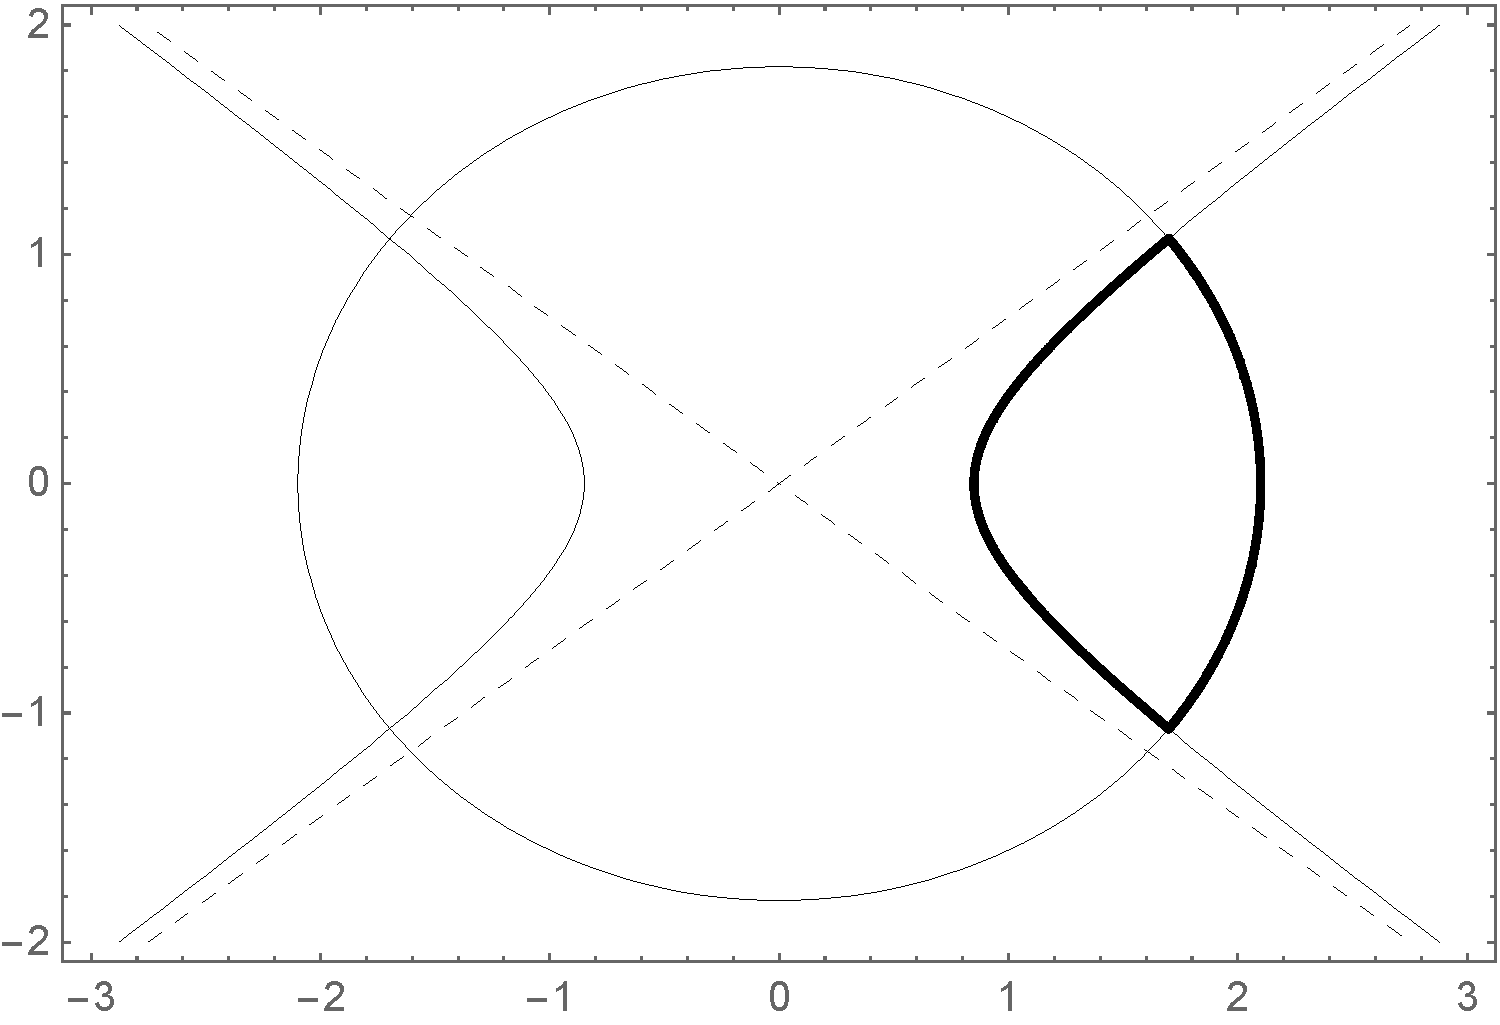
\includegraphics[width=0.8\linewidth]{right1.pdf} \\ 
        Множество $A_\varepsilon$, $\phi_0<\pi/2$
    \end{minipage}
    \hfill
    \begin{minipage}[b][][b]{0.49\linewidth}\centering
        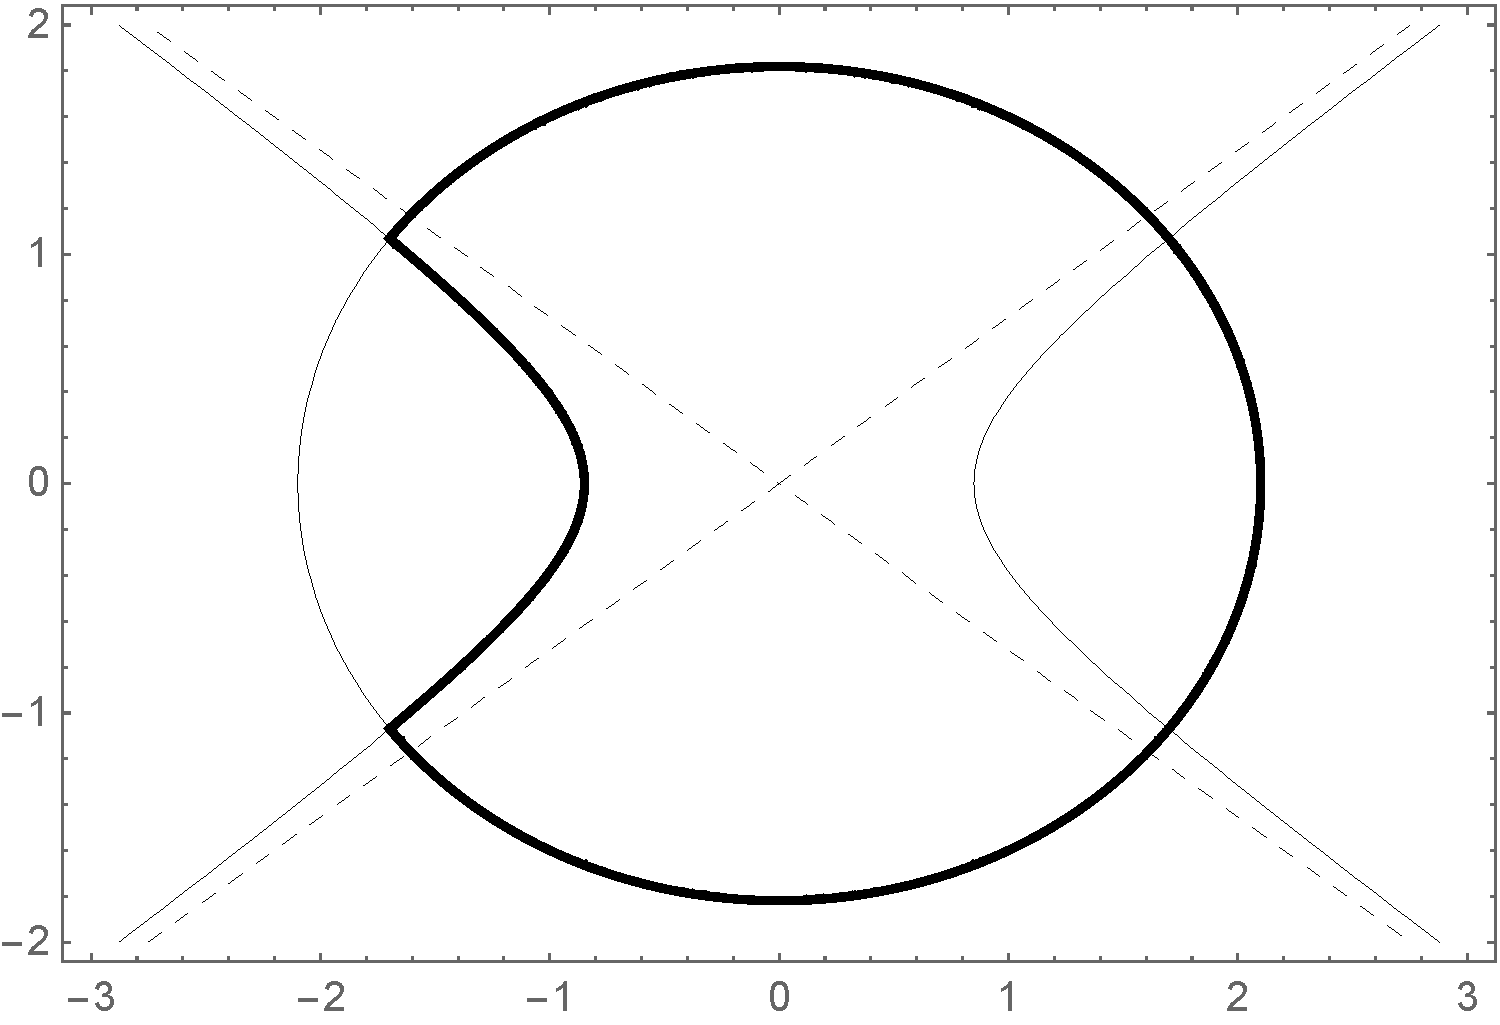
\includegraphics[width=0.8\linewidth]{left1.pdf} \\ 
        Множество $A_\varepsilon$, $\phi_0>\pi/2$
    \end{minipage}
\caption{Примеры множеств $A_\varepsilon$}
\end{figure}

\begin{figure}[ht]
\begin{minipage}{0.9\linewidth}\centering
        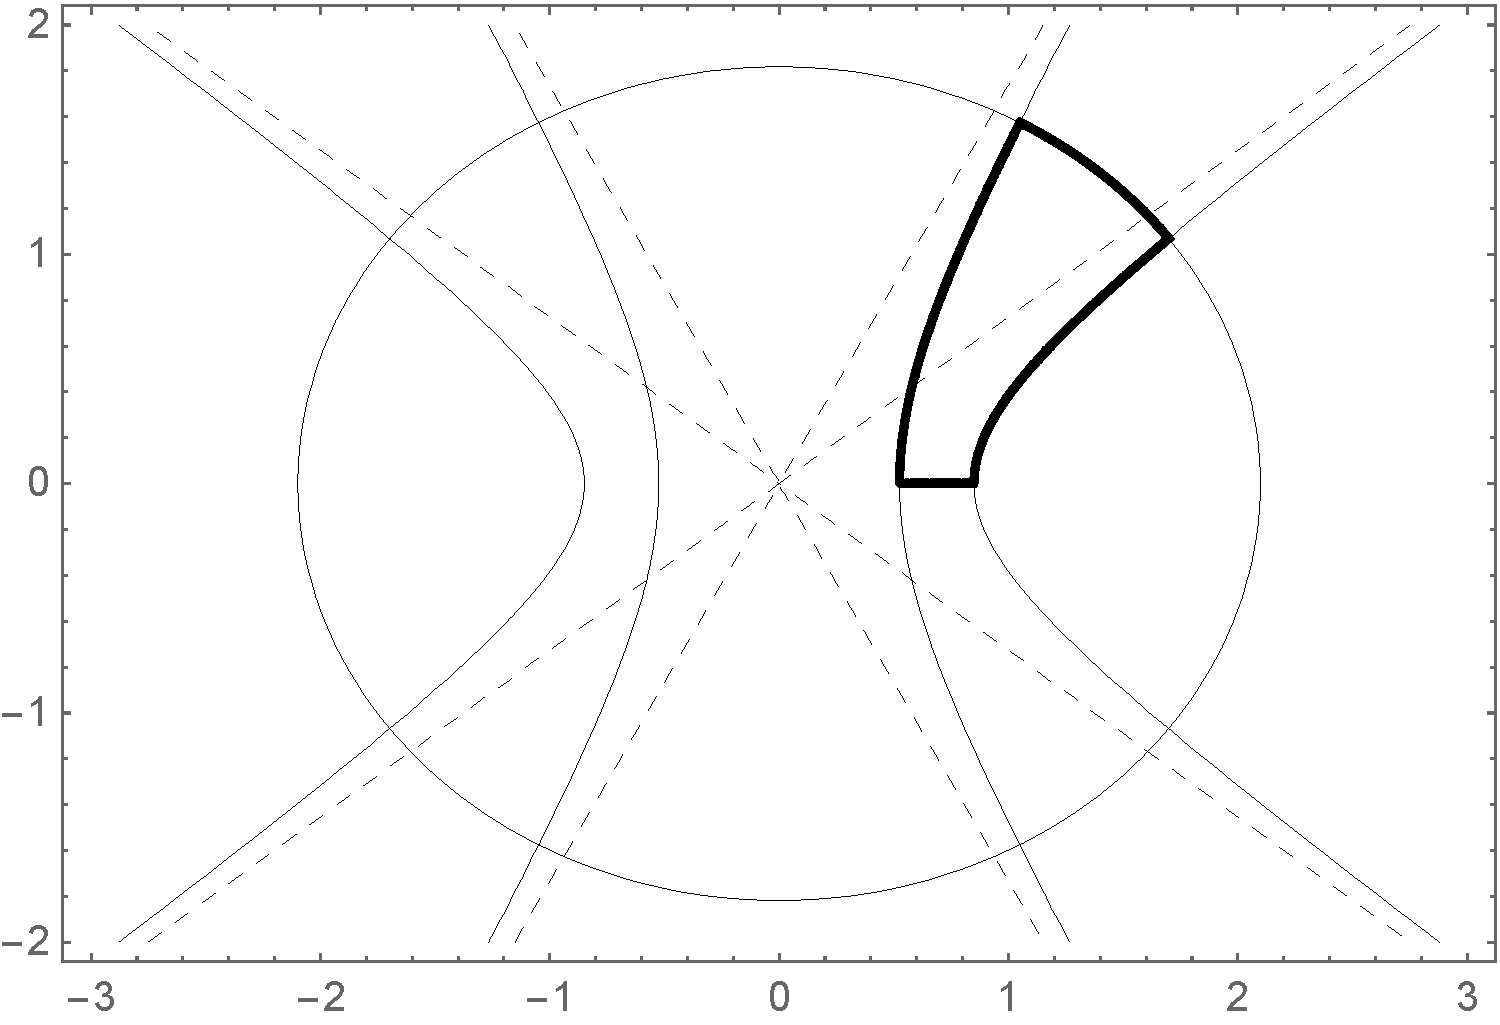
\includegraphics[width=0.8\linewidth]{up1.pdf}  
    \end{minipage}
\caption{        Множество $B_\varepsilon$, $\phi_0<\phi_1<\pi/2$}
\end{figure}

Очевидно, что с приближением величины $\varepsilon$ к 0, эллипс приближается к кругу радиуса $r_0$,
а любая гипербола~(\ref{eq:hyper}) приближается к собственным асимптотам.

Следовательно, при $\varepsilon\to 0$, область $A$ приближается к круговому сектору с величиной центрального угла $2\phi_0$, 
а область  $B$ приближается к круговому сектору с углом $\phi_1-\phi_0$. 


\subsection{Собственные функции и асимптотика собственных значений}\label{sec:ch2/sec4/subs2}
\subsubsection{Симметричная область $A_\varepsilon: \rho \in [0,\rho_0], \phi \in [-\phi_0,\phi_0]$}\label{sec:ch2/sec4/subs2/subs1}

Обозначим через $\Phi_{even}(\zeta, q, \phi), \Phi_{odd}(\zeta, q, \phi)$ четное и нечетное решения уравнения $\frac{\partial^2}{\partial \phi^2}\Phi + (\zeta - 2q\cos{2\phi})\Phi = 0$, соответственно. 
В частности, (см.~\cite{wref2})
\[
\begin{array}{ll}
    \Phi_{even}(a_n(q), q, \phi) = ce_n(\phi, q)	&
    \Phi_{odd}(a_n(q), q, \phi) = fe_n(\phi, q)\\
    \Phi_{even}(b_n(q), q, \phi) = ge_n(\phi, q)	&
    \Phi_{odd}(b_n(q), q, \phi) = se_n(\phi, q)\\
    \Phi_{even}(\lambda_{\nu+2k}(q), q, \phi) = ce_{\nu+2k}(\phi, q) 	&
    \Phi_{odd}(\lambda_{\nu+2k}(q), q, \phi) = se_{\nu+2k}(\phi, q).
\end{array}
\]

Напомним, что эллиптическая система координат имеет особенности на соединяющем фокусы отрезке. Область $A_\varepsilon$ содержит особые точки эллиптической системы координат, а именно, они находятся на отрезке $J$ с концами на правом фокусе и на вершине дуги гиперболы.
Следовательно, решение $\psi(\rho, \phi)$ и его производная должны удовлетворять условиям непрерывности \eqref{eq:disp} и \eqref{eq:grad} на  $J$.
В силу соображений раздела \ref{sec:ch2/sec2/subs1}, собственная функция  $\psi(\rho,\phi)=R(\rho) \Phi(\phi)$ оператора $\hat{H}$ в области $A_\varepsilon$ является произведением радиальной и угловой функций Матьё одинаковой четности:
$$ \psi(\rho,\phi) = \Phi_{even}(\phi) R_{even}(\rho)  
\text{ или }
 \psi(\rho,\phi) = \Phi_{odd}(\phi) R_{odd}(\rho) .  $$
%\hfill
%$\Box$
То есть, в наших обозначениях в области $A_\varepsilon$ для собственных функций $\psi_{k, m}(\rho, \phi)$ оператора   $\hat{H}$ справедливы выражения
\begin{equation}
\psi_{k, m}(\rho, \phi) = 
\left[
\begin{array}{ll}
    Ce_\nu(\rho, q) ce_\nu(\phi, q) ,   &    \text{нечетный $k \geq 1$}\\
    Se_\nu(\rho, q) se_\nu(\phi, q) ,   &    \text{четный $k \geq 2$}\\
\end{array}
\right.\label{eq:fun}
\end{equation}
с параметрами
\[
\nu = \nu_{k,m} = \nu_0+ \varepsilon^2 \nu_1 + o(\varepsilon^2),  \quad q=q_{k,m} = \dfrac{\varkappa_{k,m}^2 r_0^2 \varepsilon^2}{4},
\]
где
$$\nu_0 = \frac{\pi k}{2\phi_0}\text{\ \  и\  \  }\nu_1=\frac{\alpha_{\nu_0, m}^2}{4} \frac{\pi k \sin 2\phi_0}{\pi^2 k^2 - 4\phi_0^2}  .$$
Для соответствующих собственных  значений  $\varkappa^2_{k, m}$ справедливы равенства
\begin{equation}
\varkappa^2_{k, m} = \dfrac{\alpha_{\nu_0, m}^2}{r_0^2} +
\varepsilon^2 \dfrac{\alpha_{\nu_0, m}^3}{2 r_0^2}\dfrac{\varkappa_1 }{ \left.\frac{\partial J_{\nu_0}(u)}{\partial u}\right|_{u=\alpha_{\nu_0, m}} } + o(\varepsilon^2),\label{eq:val}
\end{equation}
где
\begin{equation*}
    \varkappa_1 = 
    \left[
\begin{array}{ll}
\frac{J_{\nu_0-2}(\alpha_{\nu_0, m})}{4(\nu_0-1)} - \frac{J_{\nu_0+2}(\alpha_{\nu_0, m})}{4(\nu_0+1)} 
  - \nu_1 \left.\frac{\partial J_\nu}{\partial \nu}\right|_{\nu=\nu_0}(\alpha_{\nu_0, m}),\qquad \text{для нечетных $k\geq 3$ ;} \\[10pt]
\frac{(\nu_0 - 2)J_{\nu_0-2}(\alpha_{\nu_0, m})   }{4\nu_0 (\nu_0-1)} -\\
\qquad - \frac{(\nu_0 + 2)J_{\nu_0+2}(\alpha_{\nu_0, m})}{4\nu_0 (\nu_0+1)}  
- \nu_1 \left.\frac{\partial J_\nu}{\partial \nu}\right|_{\nu = \nu_0}(\alpha_{\nu_0, m}), \qquad \ \ \!    \text{для четных $k \geq 2$}.        
\end{array}
\right.
\end{equation*}
Здесь $\alpha_{\nu_0,m}$ --  $m$-ый нуль функции Бесселя первого рода $J_{\nu_0}(x)$.


Нечетный и четный случаи мы рассматриваем отдельно. Сперва рассмотрим
\textit{нечетный случай}: $\psi(\rho,\phi) = R_{odd}(\rho)\Phi_{odd}(\phi)  $.

для $\nu \in \mathbb{R} \setminus \{1\}$ 
($\nu=1$ соответствует случаю  $\phi_0=\pi$, который в работе не рассматривается)
справедливо разложение ~\cite[\S 2.2]{wref12},
\begin{align}
\Phi_{odd}(\nu, &{} \phi, q)  = \notag\\
	&{} = \sin{\nu\phi} + 
	\frac{q}{4(\nu-1)} \sin{(\nu-2)\phi} -\frac{q}{4(\nu+1)} \sin{(\nu+2)\phi} + o(q). \label{eq:se}
\end{align}
Напомним, что для $\nu \in \mathbb{R} \setminus \mathbb{Z}$, $\Phi_{odd}(\nu, \phi, q) = se_\nu(\phi, q)$ и для  $\nu \in  \mathbb{Z}$, $\Phi_{odd}(\nu, \phi, q)$ является $se_\nu(\phi, q) $ или $fe_\nu(\phi, q)$ в зависимости от $\nu$, но с тем же разложением (\ref{eq:se}). 
Поэтому, для простоты будем использовать запись $se_\nu(\phi, q)$ вместо $fe_\nu(\phi, q)$, используя только разложения с точностью до $o(q)$. Этот же подход мы будем использовать в дальнейшем без явного упоминания.

Подставим  $\phi=\phi_0$ и $\nu=\nu(q) = \nu_0 + q \nu_1 + o(q)$
в граничное условие $se_{\nu(q)}(\phi_0, q)=0$ угловой функции:
 \begin{align*}
 se_{\nu(q)}(& \phi_0, q) =  \sin \nu_0 \phi_0 + \\
&{} + q \biggl( \nu_1 \phi_0 \cos \nu_0 \phi_0 + \frac{\sin(\nu_0-2)\phi_0}{4(\nu_0-1)}  -\frac{\sin(\nu_0+2)\phi_0}{4(\nu_0+1)} \biggr) + o(q) =0.
\end{align*}
Приравнивая к нулю коэффициенты при каждой степени  $q$, мы получим
\begin{equation*}
\nu_0 = \frac{\pi (2k)}{2\phi_0}, \quad \nu_1 = \frac{\pi (2k) \sin 2 \phi_0}{(\pi^2 (2k)^2 - 4\phi_0^2)}.
\end{equation*}

Рассмотрим второе граничное условие $R(\rho_0) = 0$. 
Для функции  $R(\rho)=Se_\nu(\rho, q)$
справедливо разложение в ряд по функциям Бесселя первого рода, см.~\cite[гл. VIII]{mclachlan}, поэтому:
\begin{multline*}
Se_\nu(\rho, q) \,\propto\,\,  \nu J_\nu(2\sqrt{q} \cosh{\rho})  
+q \bigl( \frac{\nu + 2}{4(\nu+1)} J_{\nu+2}(2\sqrt{q} \cosh{\rho}) - \\
- \frac{\nu - 2}{4(\nu-1)} J_{\nu-2}(2\sqrt{q} \cosh{\rho}) \bigr) + o(q).
\end{multline*}
Символ $\propto$ означает равенство с точностью до умножения на ненулевую константу.

Заметим, что $\frac{1}{\varepsilon} = \cosh \rho = \cosh \rho_0 $, тогда из  $q = \frac{\varkappa^2 r_0^2 \varepsilon^2}{4}$ следует, что $2\sqrt{q} \cosh{\rho_0} =   \varkappa r_0$. 
Для краткости обозначим $u = \varkappa r_0$. Теперь подставим  
$\nu=\nu_0 + q\nu_1 + o(q)$ в граничное условие $0 = Se_{\nu(q)}(\rho_0, q)$:
\begin{multline*}
0 = \nu_0 J_{\nu_0}(u) + q \bigl(  \nu_1 J_{\nu_0}(u) 
- \frac{\nu_0 - 2}{4(\nu_0-1)} J_{\nu_0-2}(u) + %{} \notag\\ 
\\ %&{}+
+ \frac{\nu_0 + 2}{4(\nu_0+1)} J_{\nu_0+2}(u) +
 \nu_0 \nu_1 \left.\frac{\partial J_\nu}{\partial \nu}\right|_{\nu = \nu_0}(u)
\bigr) + o(q).
\end{multline*}
После чего подставим   $u = u_0 + q u_1 + o(q)$ в последнее равенство:
\begin{multline*}
0 = \nu_0 J_{\nu_0}(u_0) + q \bigl( 
\nu_0 u_1 \left.\frac{\partial J_{\nu_0}(u)}{\partial u}\right|_{u=u_0} 
+\nu_1 J_{\nu_0}(u_0) - \frac{\nu_0 - 2}{4(\nu_0-1)} J_{\nu_0-2}(u_0) \\ 
+\frac{\nu_0 + 2}{4(\nu_0+1)} J_{\nu_0+2}(u_0) 
+ \nu_0 \nu_1 \left.\frac{\partial J_\nu}{\partial \nu}\right|_{\nu = \nu_0}(u_0)
\bigr) + o(q).
\end{multline*}
Снова приравнивая к $0$ коэффициенты при степенях  $q$, получим
\begin{align}
    u_0 =& \alpha_{\nu_0, m}, \label{eq:u0}\\
    u_1 =& \frac{1}{\left.\frac{\partial J_{\nu_0}(u)}{\partial u}\right|_{u=\alpha_{\nu_0, m}} } \biggl(
\frac{(\nu_0 - 2)J_{\nu_0-2}(\alpha_{\nu_0, m}) }{4 \nu_0(\nu_0-1)} \notag \\    
&{}- \frac{(\nu_0 + 2)J_{\nu_0+2}(\alpha_{\nu_0, m}) }{4 \nu_0(\nu_0+1)} - \nu_1 \left.\frac{\partial J_\nu}{\partial \nu}\right|_{\nu = \nu_0}(\alpha_{\nu_0, m})
    \biggr),\label{eq:u1}
\end{align}
где $\alpha_{\nu_0, m}$ --  $m$-ый нуль функции Бесселя $J_{\nu_0}(x)$. 




Из равенства $q=\frac{\varkappa^2 r_0^2 \varepsilon^2}{4}=\frac{u^2 \varepsilon^2}{4}$ можно получить выражение для собственного значения
$$\varkappa_{k, m}^2 = \frac{u^2}{r_0^2} = \frac{u_0^2}{r_0^2} + \frac{2 q u_0 u_1}{r_0^2} + o(q)= \frac{u_0^2}{r_0^2} +  \varepsilon^2 \frac{u_0^3 u_1}{2 r_0^2} + o(\varepsilon^2).$$ 
Из уравнений~(\ref{eq:u0}) и (\ref{eq:u1}) для $u_0, u_1$ верны выражения
\begin{align}
  & \nu_0 = \frac{2\pi k}{2\phi_0},   \nu_1 = \frac{2 \pi k \sin 2 \phi_0}{4 k^2\pi^2  - 4\phi_0^2},\\
   & \varkappa_{k, m}^2 = \frac{\alpha_{\nu_0, m}^2}{r_0^2} 
+  \varepsilon^2 \frac{\alpha_{\nu_0, m}^3}{2 r_0^2}\frac{1}{ \left.\frac{\partial J_{\nu_0}(u)}{\partial u}\right|_{u=\alpha_{\nu_0, m}} } \biggl(
\frac{(\nu_0 - 2)J_{\nu_0-2}(\alpha_{\nu_0, m})   }{4\nu_0 (\nu_0-1)} - \notag \\
&\qquad\qquad{}- \frac{(\nu_0 + 2)J_{\nu_0+2}(\alpha_{\nu_0, m})}{4\nu_0 (\nu_0+1)} - \nu_1 \left.\frac{\partial J_\nu}{\partial \nu}\right|_{\nu = \nu_0}(\alpha_{\nu_0, m})
    \biggr) + o(\varepsilon^2).
 \label{eq:oddSe_nueigenvalues}
 \end{align}


Теперь рассмотрим случай  $\psi(\phi, \rho) = \Phi_{even}(\phi) R_{even}(\rho)$ с \textit{четными} функциями $ \Phi_{even}(\phi) $ и $R_{even}(\rho)$. 
В силу аналогичных соображений, рассмотрим разложение четного решения:
\[
ce_\nu(\phi, q) = 	\cos{\nu\phi} + 
	\frac{q}{4(\nu-1)} \cos{(\nu-2)\phi} -\frac{q}{4(\nu+1)} \cos{(\nu+2)\phi} + o(q).
\]
Используя равенство $ce_\nu(\phi_0, q)=0$ и разложение $\nu = \nu_0 + q \nu_1 + o(q)$,
запишем разложение $ce_\nu$  по степеням $q$:
\begin{multline*}
0=ce_\nu(\phi_0, q) = 	\cos{\nu_0\phi_0}  + \\
+q \biggl(	\frac{\cos{(\nu_0-2)\phi_0}}{4(\nu_0-1)}  -\frac{\cos{(\nu_0+2)\phi_0}}{4(\nu_0+1)} - \nu_1 \phi_0 \sin \nu_0 \phi_0 \biggr) + o(q).
 \end{multline*}
Приравнивая к  $0$ коэффициенты при различных степенях  $q$, получаем
\begin{equation*}
    \nu_0 = \frac{\pi (1 + 2 k)}{2 \phi_0}, \qquad \nu_1 = \frac{\pi (1+2k) \sin 2\phi_0}{\pi^2(1+2k)^2 - 4\phi_0^2}.
\end{equation*}

Чтобы вывести формулу для  $\varkappa^2$, рассмотрим граничное условие $R(\rho_0) = 0$. 
Поскольку $R(\rho) = Ce_\nu(\rho, q)$, можно воспользоваться разложением в сумму по функциям Бесселя первого рода:
\begin{align*}
Ce_\nu(\rho, q) = & J_\nu(2\sqrt{q} \cosh{\rho}) + {}\notag \\
&{}+q \biggl( \frac{1}{4(\nu+1)} J_{\nu+2}(2\sqrt{q}\cosh{\rho}) -\frac{1}{4(\nu-1)} J_{\nu-2}(2\sqrt{q} \cosh{\rho})
\biggr) + o(q).
\end{align*}
Заметим, что $\frac{1}{\varepsilon} = \cosh \rho = \cosh \rho_0 $, тогда из  $q = \frac{\varkappa^2 r_0^2 \varepsilon^2}{4}$ следует, что $2\sqrt{q} \cosh{\rho_0} =   \varkappa r_0$. 
Обозначим для краткости $u = \varkappa r_0$. 

Подставим  $\nu = \nu_0 + q \nu_1 + o(q)$  в граничное условие $0 = Ce_{\nu(q)}(\rho_0, q)$:
\begin{equation}
    0 = 
    J_{\nu_0}(u) + q \biggl( 
    \frac{J_{\nu_0+2}(u)}{4(\nu_0+1)}  - \frac{J_{\nu_0-2}(u)}{4(\nu_0-1)}
    + \nu_1 \left.\frac{\partial J_\nu}{\partial \nu}\right|_{\nu=\nu_0}(u)
    \biggr) + o(q).\label{eq:evenae}
\end{equation}
Теперь подставим $u = u_0 + q u_1 + o(q)$  в полученное выражение~(\ref{eq:evenae}):
\begin{align*}
    &0 =  Ce_{\nu(q)}(\rho_0, q) = 
    J_{\nu_0}(u_0) + q \biggl( 
    u_1 \left.\frac{\partial J_{\nu_0} (u)}{\partial u}\right|_{u=u_0} +  \notag \\
  &\quad{}  + \frac{J_{\nu_0+2}(u_0)}{4(\nu_0+1)} - \frac{J_{\nu_0-2}(u_0)}{4(\nu_0-1)}    + \nu_1 \left.\frac{\partial J_\nu}{\partial \nu}\right|_{\nu=\nu_0}(u_0)
    \biggr) + o(q).
\end{align*}
Из равенства $0$ коэффициентов при каждой степени $q$ следует
\begin{align*}
&u_0 = \alpha_{\nu_0, m}, \\
&u_1 = \frac{1}{\left.\frac{\partial J_{\nu_0} (u)}{\partial u}\right|_{u=\alpha_{\nu_0, m}}} 
\biggl(
\frac{J_{\nu_0-2}(\alpha_{\nu_0, m})}{4(\nu_0-1)} - \frac{J_{\nu_0+2}(\alpha_{\nu_0, m})}{4(\nu_0+1)}
 - \nu_1 \left.\frac{\partial J_\nu}{\partial \nu}\right|_{\nu=\nu_0}(\alpha_{\nu_0, m})
\biggr),
\end{align*}
где $\alpha_{\nu_0, m}$ -- $m$-ый нуль функции $J_{\nu_0}(x)$.  

Как и в предыдущем случае, собственное значение
$$\varkappa_{k, m}^2 = \frac{u^2}{r_0^2} = \frac{u_0^2}{r_0^2} + \varepsilon^2 \frac{u_0^3 u_1}{2r_0^2} + o(\varepsilon^2)$$ получается подстановкой значений $u_0, u_1$:
\begin{align*}
&\nu_0 = \frac{\pi (1 + 2 k)}{2 \phi_0}, \quad \nu_1 = \frac{\pi (1+2k) \sin 2\phi_0}{\pi^2(1+2k)^2 - 4\phi_0^2},\\
&\varkappa_{k, m}^2 = \frac{\alpha_{\nu_0, m}^2}{r_0^2} + \varepsilon^2 \frac{\alpha_{\nu_0, m}^3}{2r_0^2} \frac{1}{\left.\frac{\partial J_{\nu_0} (u)}{\partial u}\right|_{u=\alpha_{\nu_0, m}}}\biggl(
\frac{J_{\nu_0-2}(\alpha_{\nu_0, m})}{4(\nu_0-1)} - \notag\\
&\qquad{} - \frac{J_{\nu_0+2}(\alpha_{\nu_0, m})}{4(\nu_0+1)}    - \nu_1 \left.\frac{\partial J_\nu}{\partial \nu}\right|_{\nu=\nu_0}(\alpha_{\nu_0, m})
\biggr) + o(\varepsilon^2).
\end{align*}


\subsubsection{Несимметричная область $B_\varepsilon:  \rho \in [0, \rho_0], \phi \in [\phi_0, \phi_1 ]$}\label{sec:ch2/sec4/subs2/subs2}

Внутренность области $B_\varepsilon$ не содержит особых точек эллиптической системы координат~(\ref{eq:coord}). Поэтому, условия непрерывности сдвига или непрерывности производной, рассмотренные для случая симметричной области (в частности, для эллипса), здесь не требуются.
Хотя эти особые точки, тем не менее, появятся на границе  $B_\varepsilon$ (а именно, они образуют горизонтальный отрезок в составе границы).

Рассмотрим собственную функцию $\psi_{k,l}(\rho,\phi) = R(\rho)\Phi(\phi)$.
Обращение  $\psi_{k,l}(\rho,\phi) $ в нуль на горизонтальном отрезке на границе  $B_\varepsilon$
подразумевает, что $\psi_{k,l}(\rho,\phi)$ может быть представлена в виде
\[
\psi(\rho,\phi) = 
    \left(
    \Phi_{even}(\phi_0) \Phi_{odd}(\phi) - \Phi_{even}(\phi) \Phi_{odd}(\phi_0) 
    \right) R_{odd}(\rho).
\]

{\em Далее следует основной результат текущего подраздела.}
В области  $B_\varepsilon$ для собственных функций $\psi_{k, m}(\rho, \phi)$ и собственных значений $\varkappa^2_{k, m}$ оператора $\hat{H}$ справедливы выражения

\begin{align}
&\psi_{k, m}(\rho, \phi) = 
    Se_\nu(\rho, q) \biggl( ce_\nu(\phi_0, q) se_\nu(\phi, q) -ce_\nu(\phi, q) se_\nu(\phi_0, q) \biggr) ,  \label{eq:funB}
\end{align}
с параметрами
\begin{align*}    
    & q=q_{k,m} = \frac{\varkappa_{k,m}^2 r_0^2 \varepsilon^2}{4}, \\ 
&\nu = \nu_{k,m} = \frac{\pi k}{\phi_1-\phi_0} +\varepsilon^2 \frac{\alpha_{\nu_0, m}^2}{4} \frac{\pi k (\sin 2\phi_1 - \sin 2 \phi_0)}{\pi^2k^2-(\phi_1-\phi_0)^2} + o(\varepsilon^2) ,  
\end{align*}
где
\begin{align*}
& \nu_0 = \frac{\pi k}{\phi_1-\phi_0},\text{\ \ и \ \ }
\nu_1= \frac{\pi k (\sin 2\phi_1 - \sin 2 \phi_0)}{\pi^2k^2-(\phi_1-\phi_0)^2} .
\end{align*}
Для соответствующих собственных значений справедливы равенства
\begin{align}
\varkappa_{k, m}^2 ={}& \frac{\alpha_{\nu_0, m}^2}{r_0^2} +  \varepsilon^2 \frac{\alpha_{\nu_0, m}^3}{2 r_0^2}\frac{1}{ \left.\frac{\partial J_{\nu_0}(u)}{\partial u}\right|_{u=\alpha_{\nu_0, m}} }  
 \biggl(\frac{(\nu_0 - 2)J_{\nu_0-2}(\alpha_{\nu_0, m})   }{4\nu_0 (\nu_0-1)} 
\notag \\ 
&{}- \frac{(\nu_0 + 2)J_{\nu_0+2}(\alpha_{\nu_0, m})}{4\nu_0 (\nu_0+1)} 
- \nu_1 \left.\frac{\partial J_\nu}{\partial \nu}\right|_{\nu = \nu_0}(\alpha_{\nu_0, m})
    \biggr) + o(\varepsilon^2).\label{eq:valB}
\end{align}
Здесь $\alpha_{\nu_0,m}$ -- $m$-ый нуль функции Бесселя первого рода $J_{\nu_0}(x)$.


Мы хотим найти решение углового решения в виде
\begin{multline*}
\Phi(\phi, q) = \Phi_{even}(\phi_0) \Phi_{odd}(\phi) - \Phi_{even}(\phi) \Phi_{odd}(\phi_0)  = \\
=ce_\nu(\phi_0, q) se_\nu(\phi, q) - ce_\nu(\phi, q) se_\nu(\phi_0, q).
\end{multline*}

 
Подстановим $\nu(q) = \nu_0 + q \nu_1 + o(q)$
в граничное условие  $\Phi(\phi_1, q) = 0$
и из разложения функций $ce_\nu(\phi, q)$ и $se_\nu(\phi, q)$, в ряды по степеням  $q$
 получим
\begin{multline*}
0=\Phi(\phi_1, q) = ce_\nu(\phi_0, q) se_\nu(\phi_1, q) -ce_\nu(\phi_1, q) se_\nu(\phi_0, q) = \\
= \sin \nu_0 (\phi_1 - \phi_0) +q \biggl(
\frac{1}{4(\nu_0+1)}  \sin{(2 \phi_0 + \nu_0(\phi_0-\phi_1))}+  \\
+\frac{1}{4(\nu_0+1)} \sin{(\nu_0(\phi_0-\phi_1)-2\phi_1)} - \\
-\frac{1}{2(\nu_0-1)}\cos{(\phi_0 + \phi_1)}\sin{(\nu-1)(\phi_0-\phi_1)} -\\
- \nu_1 (\phi_0 - \phi_1) \cos{\nu_0(\phi_0-\phi_1)} \biggr) + o(q).
\end{multline*}
Следовательно, 
\begin{equation*}
    \nu_0 = \frac{\pi k}{\phi_1-\phi_0}, \qquad \nu_1 = \frac{\pi k (\sin 2\phi_1 - \sin 2 \phi_0)}{\pi^2k^2-(\phi_1-\phi_0)^2}.
\end{equation*}

Из соображений, аналогичных тем, что были проведены для  $\psi_{k, m}(\rho, \phi) = \Phi_{odd}(\phi) R_{odd}(\rho)$ из предыдущего подраздела,
мы получаем разложение радиальной функции и соответствующих собственных значений:
\begin{align*}
    \varkappa_{k, m}^2 ={}& \frac{\alpha_{\nu_0, m}^2}{r_0^2} +  \varepsilon^2 \frac{\alpha_{\nu_0, m}^3}{2 r_0^2}\frac{1}{ \left.\frac{\partial J_{\nu_0}(u)}{\partial u}\right|_{u=\alpha_{\nu_0, m}} }\biggl(\frac{(\nu_0 - 2)J_{\nu_0-2}(\alpha_{\nu_0, m})   }{4\nu_0 (\nu_0-1)} \notag \\
&{}- \frac{(\nu_0 + 2)J_{\nu_0+2}(\alpha_{\nu_0, m})}{4\nu_0 (\nu_0+1)}  - \nu_1 \left.\frac{\partial J_\nu}{\partial \nu}\right|_{\nu = \nu_0}(\alpha_{\nu_0, m})
    \biggr) + o(\varepsilon^2).
\end{align*}

\subsection{Особые случаи}\label{sec:ch2/sec4/subs3}
\subsubsection{$A_\varepsilon$ для $\phi_0=\pi/2$}\label{sec:ch2/sec4/subs3/subs1}


Для $\nu\ne 1$ формулы для собственных функций и собственных значений, см. уравнения (\ref{eq:fun}) и (\ref{eq:val}), верны. Единственным исключением является случай  $\nu=\nu_0=1$.
Для $\nu=\nu_0=1$ для четного решения справедливо разложение (см. \cite[Subsect.~20.2.27]{wref2}):
\begin{equation*}
ce_1(\phi, q) = 	\cos{\phi}  - \frac{q}{8} \cos{3\phi} + o(q),
 \end{equation*}
для которого граничное условие  $ce_1(\phi_0, q)=0$ выполняется. 
Рассмотрим второе граничное условие $R(\rho_0) = 0$.
Для $R(\rho) = Ce_1(\rho, q)$ существует разложение по функциям Бесселя первого рода:
\begin{equation*}
Ce_1(\rho, q) = J_1(2\sqrt{q} \cosh{\rho}) + \frac{q}{8} J_3(2\sqrt{q}\cosh{\rho}) + o(q).
\end{equation*}
Из подстановок $\cosh\rho = \cosh\rho_0 =  \frac{1}{\varepsilon}$ и $q = \frac{\varkappa^2 r_0^2 \varepsilon^2}{4}$ следует равенство
$2\sqrt{q} \cosh{\rho_0} = 2 \frac{\varkappa r_0 \varepsilon}{2} \frac{1}{\varepsilon} = \varkappa r_0$. Для краткости $\varkappa r_0$ обозначим через $u$. 

Подставим $\nu = 1$ в граничное условие $0 = Ce_1(\rho_0, q)$ и рассмотрим разложение в ряд по степеням   $q$:
\begin{equation*}
    0 = J_1(u) + q \left( \frac{J_3(u)}{8} \right) + o(q).
\end{equation*}
Подстановкой  $u = u_0 + q u_1 + o(q)$ получим:
\begin{equation*}
    0 = 
    J_1(u_0) + q \left( 
    u_1 \left.\frac{\partial J_1 (u)}{\partial u}\right|_{u=u_0}
    + \frac{J_3(u_0)}{8}
    \right) + o(q).
\end{equation*}
Поэтому, 
\begin{equation*}
u_0 = \alpha_{1, m}, \qquad u_1 = 
\frac{ - J_3(\alpha_{1, m}) }{8\left.
\frac{\partial J_1 (u)}{\partial u}\right|_{u=\alpha_{1, m}}},
\end{equation*}
где $\alpha_{1, m}$ -- $m$-ый нуль функции Бесселя  $J_1(x)$. По аналогии с предыдущим случаем,
собственное значение $\varkappa_{k, m}^2 = \frac{u^2}{r_0^2} = \frac{u_0^2}{r_0^2} + \varepsilon^2 \frac{u_0^3 u_1}{2r_0^2} + o(\varepsilon^2)$ получается из подстановки величин  $u_0, u_1$:
\begin{align}
   & \varkappa_{k, m}^2 = \frac{\alpha_{1, m}^2}{r_0^2} - \varepsilon^2 \frac{\alpha_{1, m}^3}{16r_0^2} 
    \frac{J_3(\alpha_{1, m})}{\left.\frac{\partial J_1 (u)}{\partial u}\right|_{u=\alpha_{1, m}}} 
    + o(\varepsilon^2), \label{eq:valS1}
    \end{align}



\subsubsection{$B_\varepsilon$: $\phi_0=0, \phi_1=\pi$ и $\phi_0=0, \phi_1=\pi/2$}\label{sec:ch2/sec4/subs3/subs2}


Хотя $\phi_0=0, \phi_1=\pi/2$ является особенным случаем при $k=1$,
несложно проверить, что уравнения (\ref{eq:funB}) и (\ref{eq:valB}) выполняются.

Для  $\phi_0=0, \phi_1=\pi$
особенным является случай  $k=1$ (следовательно, $\nu_0=1$). 
Для остальных величин $k$ равенства (\ref{eq:funB}) и (\ref{eq:valB}) справедливы.
Теперь предположим $k=1$ (и $\nu=\nu_0 = 1$).
Тогда для соответствующего нечетного решения углового уравнения справедливо разложение  (см. \cite[Subsect.~20.2.27]{wref2})
\begin{equation*}
se_1(\phi, q) = 	\sin{\phi}  - 	\frac{q}{8} \sin{3\phi} + o(q),
 \end{equation*}
для которого выполняется граничное условие $se_1(\phi_0, q)=0$. 
Теперь рассмотрим второе граничное условие $R(\rho_0) = 0$. 
Для функции $R(\rho) = Se_1(\rho, q)$ справедливо разложение по функциям Бесселя первого рода:
\begin{equation*}
Se_1(\rho, q) = J_1(2\sqrt{q} \cosh{\rho}) + \frac{3 q}{8} J_3(2\sqrt{q}\cosh{\rho}) + o(q).
\end{equation*}
Подставим $\cosh \rho = \cosh \rho_0 =\frac{1}{\varepsilon}$.
Тогда из $q = \frac{\varkappa^2 r_0^2 \varepsilon^2}{4}$ следует равенство
$2\sqrt{q} \cosh{\rho_0} =  \varkappa r_0$.

Для краткости положим $u = \varkappa r_0$ .
Подставим $\nu = 1$ в граничное условие радиальной функции и разложим ее в ряд степенной ряд по $q$:
\begin{equation*}
    0 = Se_1(\rho_0, q) = 
    J_1(u) + q  \frac{3 J_3(u)}{8} + o(q).
\end{equation*}
Теперь подставим $u = u_0 + q u_1 + o(q)$:
\begin{align*}
    0 = Se_1(\rho_0, q) =    J_1(u_0) + q \left( 
    u_1 \left.\frac{\partial J_1 (u)}{\partial u}\right|_{u=u_0}
    + \frac{3 J_3(u_0)}{8}
    \right) + o(q).
\end{align*}
Отсюда 
\begin{equation*}
u_0 = \alpha_{1, m}, \qquad u_1 = 
\frac{ - 3 J_3(\alpha_{1, m}) }{8\left.
\frac{\partial J_1 (u)}{\partial u}\right|_{u=\alpha_{1, m}}},
\end{equation*}
где $\alpha_{1, m}$ -- $m$-ый нуль функции $J_1(x)$. 

Наконец, как в предыдущем случае, подстановкой $u_0, u_1$ в $\varkappa_{1, m}^2 = \frac{u^2}{r_0^2} = \frac{u_0^2}{r_0^2} + \varepsilon^2 \frac{u_0^3 u_1}{2r_0^2} + o(\varepsilon^2)$, получим выражение для собственного значения:
\begin{align}
    \varkappa_{1, m}^2& = \frac{\alpha_{1, m}^2}{r_0^2} - \varepsilon^2 \frac{3\alpha_{1, m}^3}{16r_0^2} 
    \frac{J_3(\alpha_{1, m})}{\left.\frac{\partial J_1 (u)}{\partial u}\right|_{u=\alpha_{1, m}}} 
    + o(\varepsilon^2).  \label{eq:valS2}
\end{align}



\FloatBarrier
